\documentclass[]{article}
\usepackage{lmodern}
\usepackage{amssymb,amsmath}
\usepackage{ifxetex,ifluatex}
\usepackage{fixltx2e} % provides \textsubscript
\ifnum 0\ifxetex 1\fi\ifluatex 1\fi=0 % if pdftex
  \usepackage[T1]{fontenc}
  \usepackage[utf8]{inputenc}
\else % if luatex or xelatex
  \ifxetex
    \usepackage{mathspec}
  \else
    \usepackage{fontspec}
  \fi
  \defaultfontfeatures{Ligatures=TeX,Scale=MatchLowercase}
\fi
% use upquote if available, for straight quotes in verbatim environments
\IfFileExists{upquote.sty}{\usepackage{upquote}}{}
% use microtype if available
\IfFileExists{microtype.sty}{%
\usepackage{microtype}
\UseMicrotypeSet[protrusion]{basicmath} % disable protrusion for tt fonts
}{}
\usepackage[margin=1in]{geometry}
\usepackage{hyperref}
\hypersetup{unicode=true,
            pdftitle={考古学のためのデータビジュアライゼーション},
            pdfauthor={@ishiijunpei},
            pdfborder={0 0 0},
            breaklinks=true}
\urlstyle{same}  % don't use monospace font for urls
\usepackage{color}
\usepackage{fancyvrb}
\newcommand{\VerbBar}{|}
\newcommand{\VERB}{\Verb[commandchars=\\\{\}]}
\DefineVerbatimEnvironment{Highlighting}{Verbatim}{commandchars=\\\{\}}
% Add ',fontsize=\small' for more characters per line
\usepackage{framed}
\definecolor{shadecolor}{RGB}{248,248,248}
\newenvironment{Shaded}{\begin{snugshade}}{\end{snugshade}}
\newcommand{\AlertTok}[1]{\textcolor[rgb]{0.94,0.16,0.16}{#1}}
\newcommand{\AnnotationTok}[1]{\textcolor[rgb]{0.56,0.35,0.01}{\textbf{\textit{#1}}}}
\newcommand{\AttributeTok}[1]{\textcolor[rgb]{0.77,0.63,0.00}{#1}}
\newcommand{\BaseNTok}[1]{\textcolor[rgb]{0.00,0.00,0.81}{#1}}
\newcommand{\BuiltInTok}[1]{#1}
\newcommand{\CharTok}[1]{\textcolor[rgb]{0.31,0.60,0.02}{#1}}
\newcommand{\CommentTok}[1]{\textcolor[rgb]{0.56,0.35,0.01}{\textit{#1}}}
\newcommand{\CommentVarTok}[1]{\textcolor[rgb]{0.56,0.35,0.01}{\textbf{\textit{#1}}}}
\newcommand{\ConstantTok}[1]{\textcolor[rgb]{0.00,0.00,0.00}{#1}}
\newcommand{\ControlFlowTok}[1]{\textcolor[rgb]{0.13,0.29,0.53}{\textbf{#1}}}
\newcommand{\DataTypeTok}[1]{\textcolor[rgb]{0.13,0.29,0.53}{#1}}
\newcommand{\DecValTok}[1]{\textcolor[rgb]{0.00,0.00,0.81}{#1}}
\newcommand{\DocumentationTok}[1]{\textcolor[rgb]{0.56,0.35,0.01}{\textbf{\textit{#1}}}}
\newcommand{\ErrorTok}[1]{\textcolor[rgb]{0.64,0.00,0.00}{\textbf{#1}}}
\newcommand{\ExtensionTok}[1]{#1}
\newcommand{\FloatTok}[1]{\textcolor[rgb]{0.00,0.00,0.81}{#1}}
\newcommand{\FunctionTok}[1]{\textcolor[rgb]{0.00,0.00,0.00}{#1}}
\newcommand{\ImportTok}[1]{#1}
\newcommand{\InformationTok}[1]{\textcolor[rgb]{0.56,0.35,0.01}{\textbf{\textit{#1}}}}
\newcommand{\KeywordTok}[1]{\textcolor[rgb]{0.13,0.29,0.53}{\textbf{#1}}}
\newcommand{\NormalTok}[1]{#1}
\newcommand{\OperatorTok}[1]{\textcolor[rgb]{0.81,0.36,0.00}{\textbf{#1}}}
\newcommand{\OtherTok}[1]{\textcolor[rgb]{0.56,0.35,0.01}{#1}}
\newcommand{\PreprocessorTok}[1]{\textcolor[rgb]{0.56,0.35,0.01}{\textit{#1}}}
\newcommand{\RegionMarkerTok}[1]{#1}
\newcommand{\SpecialCharTok}[1]{\textcolor[rgb]{0.00,0.00,0.00}{#1}}
\newcommand{\SpecialStringTok}[1]{\textcolor[rgb]{0.31,0.60,0.02}{#1}}
\newcommand{\StringTok}[1]{\textcolor[rgb]{0.31,0.60,0.02}{#1}}
\newcommand{\VariableTok}[1]{\textcolor[rgb]{0.00,0.00,0.00}{#1}}
\newcommand{\VerbatimStringTok}[1]{\textcolor[rgb]{0.31,0.60,0.02}{#1}}
\newcommand{\WarningTok}[1]{\textcolor[rgb]{0.56,0.35,0.01}{\textbf{\textit{#1}}}}
\usepackage{longtable,booktabs}
\usepackage{graphicx,grffile}
\makeatletter
\def\maxwidth{\ifdim\Gin@nat@width>\linewidth\linewidth\else\Gin@nat@width\fi}
\def\maxheight{\ifdim\Gin@nat@height>\textheight\textheight\else\Gin@nat@height\fi}
\makeatother
% Scale images if necessary, so that they will not overflow the page
% margins by default, and it is still possible to overwrite the defaults
% using explicit options in \includegraphics[width, height, ...]{}
\setkeys{Gin}{width=\maxwidth,height=\maxheight,keepaspectratio}
\IfFileExists{parskip.sty}{%
\usepackage{parskip}
}{% else
\setlength{\parindent}{0pt}
\setlength{\parskip}{6pt plus 2pt minus 1pt}
}
\setlength{\emergencystretch}{3em}  % prevent overfull lines
\providecommand{\tightlist}{%
  \setlength{\itemsep}{0pt}\setlength{\parskip}{0pt}}
\setcounter{secnumdepth}{0}
% Redefines (sub)paragraphs to behave more like sections
\ifx\paragraph\undefined\else
\let\oldparagraph\paragraph
\renewcommand{\paragraph}[1]{\oldparagraph{#1}\mbox{}}
\fi
\ifx\subparagraph\undefined\else
\let\oldsubparagraph\subparagraph
\renewcommand{\subparagraph}[1]{\oldsubparagraph{#1}\mbox{}}
\fi

%%% Use protect on footnotes to avoid problems with footnotes in titles
\let\rmarkdownfootnote\footnote%
\def\footnote{\protect\rmarkdownfootnote}

%%% Change title format to be more compact
\usepackage{titling}

% Create subtitle command for use in maketitle
\providecommand{\subtitle}[1]{
  \posttitle{
    \begin{center}\large#1\end{center}
    }
}

\setlength{\droptitle}{-2em}

  \title{考古学のためのデータビジュアライゼーション}
    \pretitle{\vspace{\droptitle}\centering\huge}
  \posttitle{\par}
    \author{@ishiijunpei}
    \preauthor{\centering\large\emph}
  \postauthor{\par}
    \date{}
    \predate{}\postdate{}
  

\begin{document}
\maketitle

\href{https://ishiijunpei.github.io/2019datasience/.}{``発表スライド''}

\begin{Shaded}
\begin{Highlighting}[]
\CommentTok{# パッケージ読み込み}
\KeywordTok{library}\NormalTok{(tidyverse)}
\KeywordTok{library}\NormalTok{(ggthemes)}
\KeywordTok{library}\NormalTok{(knitr)}
\KeywordTok{library}\NormalTok{(rmarkdown)}
\KeywordTok{library}\NormalTok{(revealjs)}
\end{Highlighting}
\end{Shaded}

\subsection{覚えるべき用語}

\subsubsection{連続量}

数字で表される属性です。土器の口径、器高、石器の刃部長や重量などです。

\subsubsection{離散量}

何らかの分類がなされ、記号で表される属性です。土器の分類、石器の器種などです。

\subsection{連続量と離散量の組み合わせによる可視化手法}

\begin{itemize}
\tightlist
\item
  連続量     ヒストグラム
\item
  連続量×連続量 散布図
\item
  離散量     棒グラフ
\item
  離散量×離散量 積上げ棒グラフ、ファセット棒グラフ
\item
  離散量×連続量 ファセットヒストグラム、箱ひげ図 
\end{itemize}

\subsection{連続量と離散量〜法量と土器分類の関係〜}

以下の手順でダミーデータを生成します。

\begin{Shaded}
\begin{Highlighting}[]
\CommentTok{# irisデータ読み込み}
\NormalTok{data<-iris}
\CommentTok{#ダミーデータ生成}
\NormalTok{pot<-data[,}\KeywordTok{c}\NormalTok{(}\DecValTok{1}\NormalTok{,}\DecValTok{2}\NormalTok{,}\DecValTok{5}\NormalTok{)]}
\KeywordTok{colnames}\NormalTok{(pot)<-}\KeywordTok{c}\NormalTok{(}\StringTok{"器高"}\NormalTok{,}\StringTok{"口径"}\NormalTok{,}\StringTok{"分類"}\NormalTok{)}
\NormalTok{pot}\OperatorTok{$}\NormalTok{分類<-}\KeywordTok{factor}\NormalTok{(pot}\OperatorTok{$}\NormalTok{分類,}\DataTypeTok{levels=}\KeywordTok{c}\NormalTok{(}\StringTok{"setosa"}\NormalTok{,}\StringTok{"versicolor"}\NormalTok{,}\StringTok{"virginica"}\NormalTok{),}
    \DataTypeTok{labels=}\KeywordTok{c}\NormalTok{(}\StringTok{"A型"}\NormalTok{,}\StringTok{"B型"}\NormalTok{,}\StringTok{"C型"}\NormalTok{))}
\NormalTok{pot}\OperatorTok{$}\NormalTok{器高<-pot}\OperatorTok{$}\NormalTok{器高}\OperatorTok{*}\DecValTok{7}
\NormalTok{pot}\OperatorTok{$}\NormalTok{口径<-pot}\OperatorTok{$}\NormalTok{口径}\OperatorTok{*}\DecValTok{10}
\NormalTok{pot}\OperatorTok\KeywordTok{head}\NormalTok{()}\OperatorTok\KeywordTok{kable}\NormalTok{()}
\end{Highlighting}
\end{Shaded}

\begin{longtable}[]{@{}ccl@{}}
\toprule
器高 & 口径 & 分類\tabularnewline
\midrule
\endhead
35.7 & 35 & A型\tabularnewline
34.3 & 30 & A型\tabularnewline
32.9 & 32 & A型\tabularnewline
32.2 & 31 & A型\tabularnewline
35.0 & 36 & A型\tabularnewline
37.8 & 39 & A型\tabularnewline
\bottomrule
\end{longtable}

土器の口径をx軸、器高をy軸にとって散布図を描き、法量と土器分類の関係を調べるケースを想定しています。
下のような散布図により、「A型」は「B型」や「C」型と区別できそうだ、などと判断するわけです。

\begin{Shaded}
\begin{Highlighting}[]
\NormalTok{pot}\OperatorTok
\StringTok{    }\KeywordTok{ggplot}\NormalTok{(}\KeywordTok{aes}\NormalTok{(}\DataTypeTok{x=}\NormalTok{口径,}\DataTypeTok{y=}\NormalTok{器高,}\DataTypeTok{colour=}\NormalTok{分類))}\OperatorTok{+}
\StringTok{        }\KeywordTok{geom_point}\NormalTok{()}\OperatorTok{+}
\StringTok{        }\KeywordTok{scale_colour_ptol}\NormalTok{()}\OperatorTok{+}
\StringTok{        }\KeywordTok{theme_minimal}\NormalTok{()}
\end{Highlighting}
\end{Shaded}

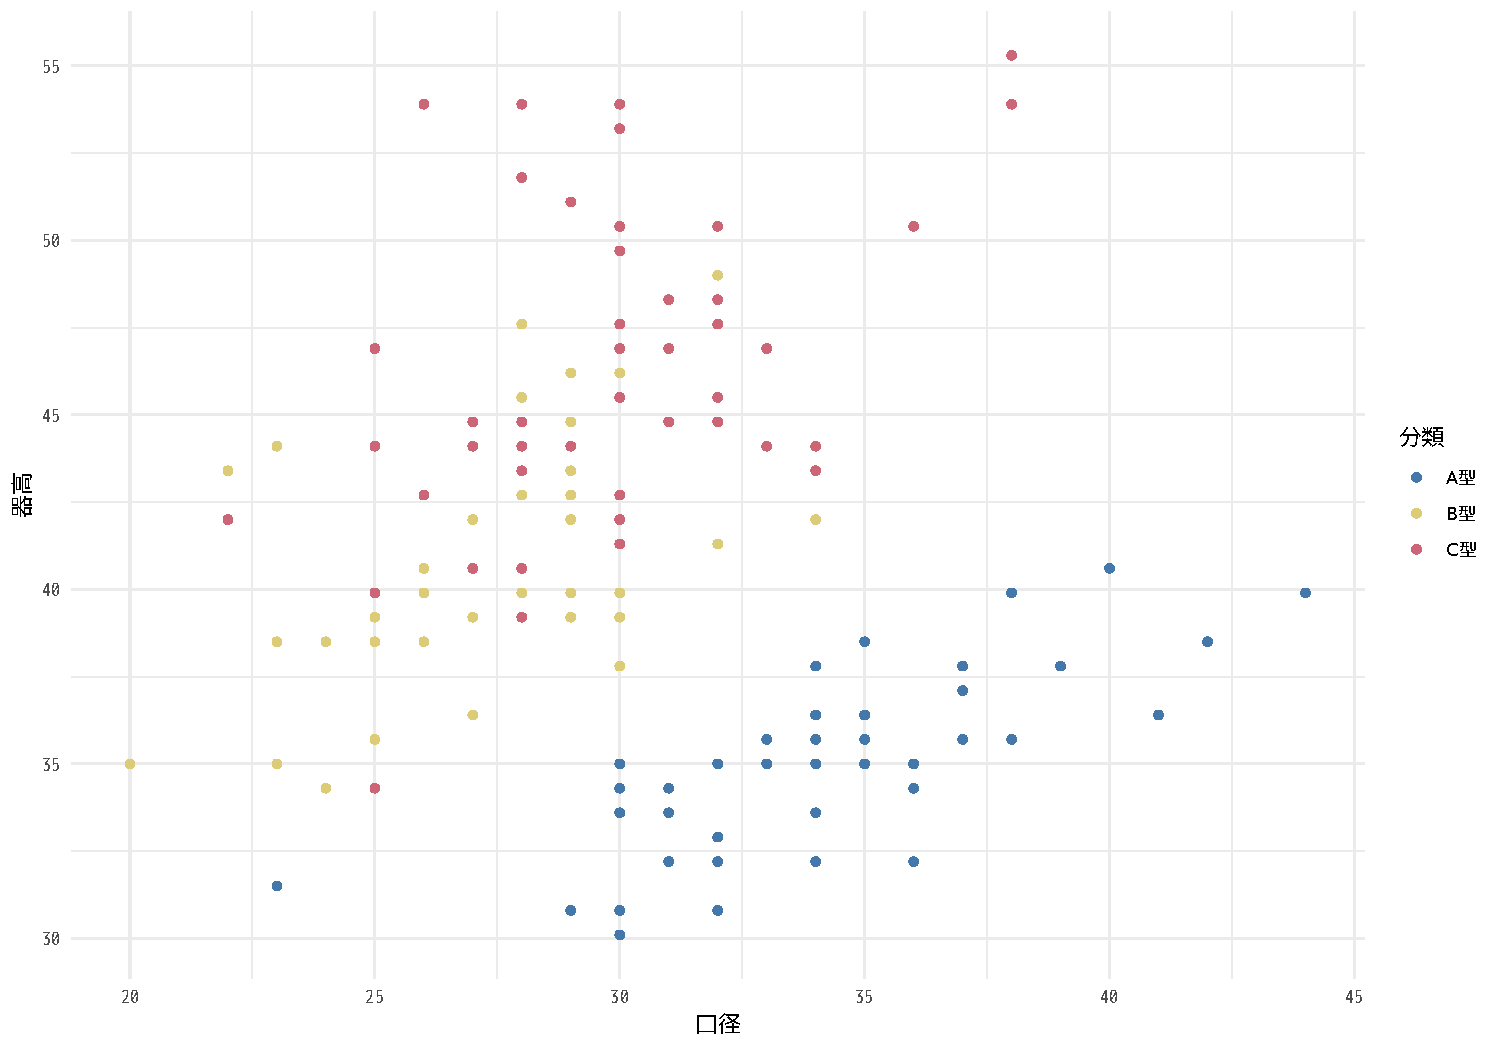
\includegraphics{document_files/figure-latex/unnamed-chunk-3-1.pdf}

\subsection{一変量ずつ分析する}

複数の連続量の分布を散布図を用いて可視化する前に、一変量ずつ分布を確認することが必要です。
連続量と離散量の組み合わせで可視化する場合には以下のような方法があります。

\subsubsection{ヒストグラム}

\begin{Shaded}
\begin{Highlighting}[]
\NormalTok{p<-pot}\OperatorTok
\StringTok{    }\KeywordTok{ggplot}\NormalTok{(}\KeywordTok{aes}\NormalTok{(}\DataTypeTok{x=}\NormalTok{口径,}\DataTypeTok{fill=}\NormalTok{分類))}\OperatorTok{+}
\StringTok{        }\KeywordTok{geom_histogram}\NormalTok{()}\OperatorTok{+}
\StringTok{        }\KeywordTok{scale_fill_ptol}\NormalTok{()}\OperatorTok{+}
\StringTok{        }\KeywordTok{facet_wrap}\NormalTok{(}\OperatorTok{~}\NormalTok{分類,}\DataTypeTok{ncol=}\DecValTok{1}\NormalTok{,}\DataTypeTok{scales=}\StringTok{"free_y"}\NormalTok{)}\OperatorTok{+}
\StringTok{        }\KeywordTok{theme_minimal}\NormalTok{()}
\KeywordTok{print}\NormalTok{(p)}
\end{Highlighting}
\end{Shaded}

\begin{verbatim}
## `stat_bin()` using `bins = 30`. Pick better value with `binwidth`.
\end{verbatim}

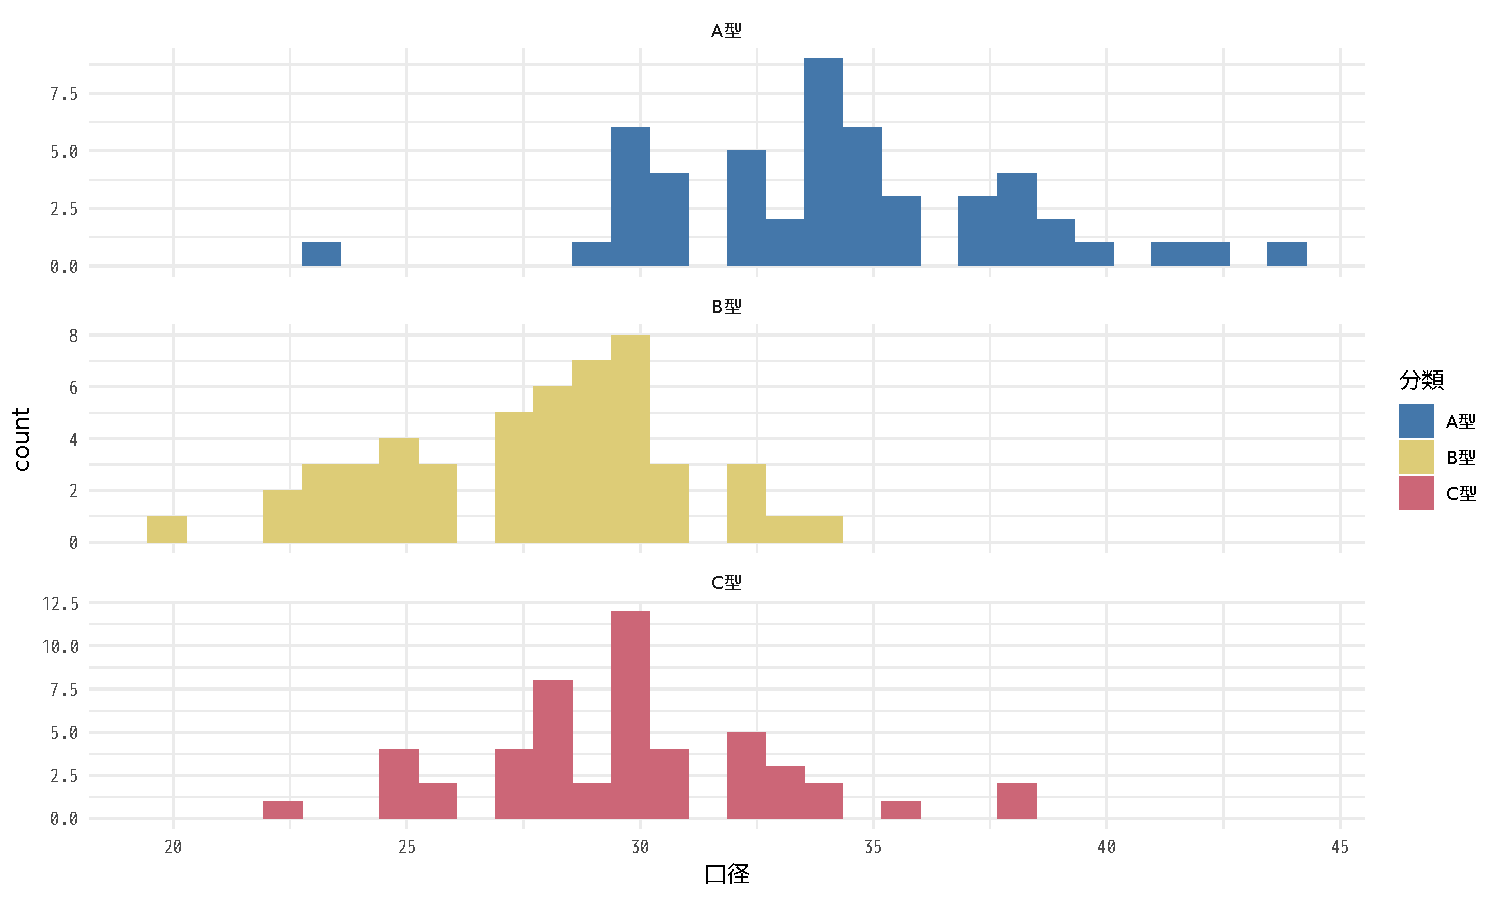
\includegraphics{document_files/figure-latex/unnamed-chunk-4-1.pdf}

\subsubsection{密度図}

\begin{Shaded}
\begin{Highlighting}[]
\NormalTok{p<-pot}\OperatorTok
\StringTok{    }\KeywordTok{ggplot}\NormalTok{(}\KeywordTok{aes}\NormalTok{(}\DataTypeTok{x=}\NormalTok{口径,}\DataTypeTok{fill=}\NormalTok{分類,}\DataTypeTok{alpha=}\FloatTok{0.7}\NormalTok{))}\OperatorTok{+}
\StringTok{        }\KeywordTok{geom_density}\NormalTok{()}\OperatorTok{+}
\StringTok{        }\KeywordTok{scale_fill_ptol}\NormalTok{()}\OperatorTok{+}
\StringTok{        }\KeywordTok{theme_minimal}\NormalTok{()}
\KeywordTok{print}\NormalTok{(p)}
\end{Highlighting}
\end{Shaded}

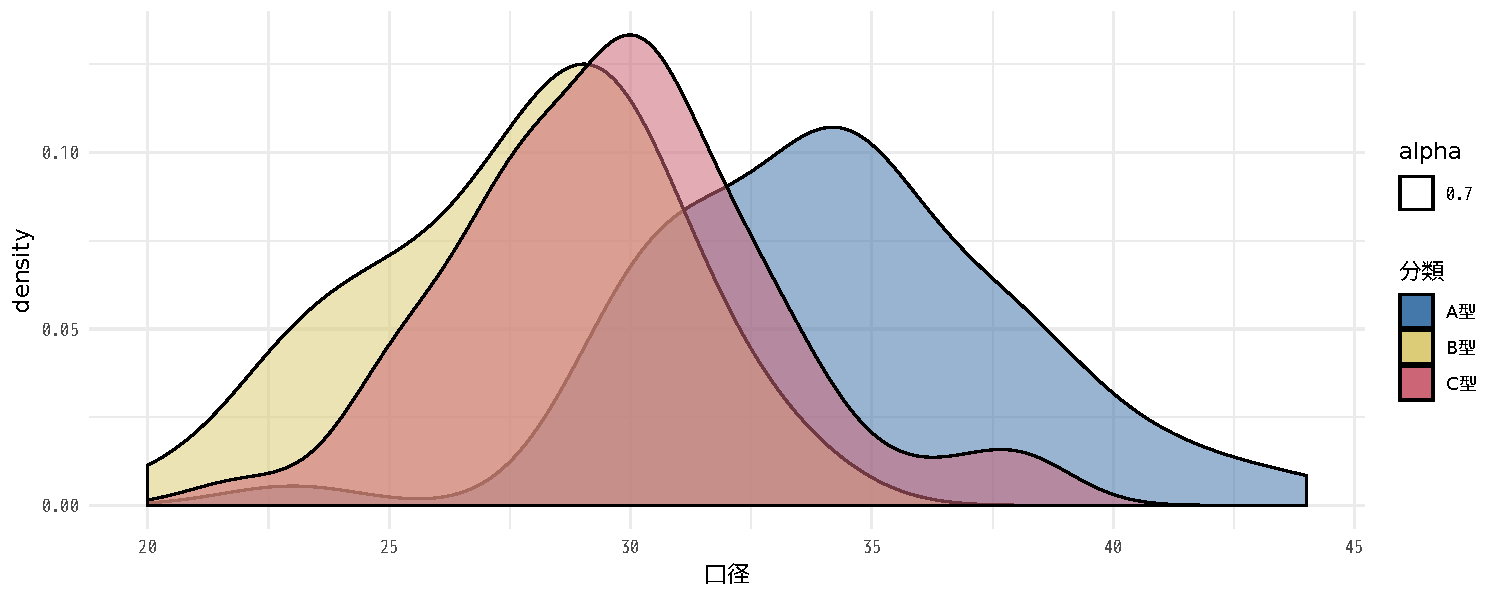
\includegraphics{document_files/figure-latex/unnamed-chunk-5-1.pdf}

\subsubsection{箱ひげ図}

\begin{Shaded}
\begin{Highlighting}[]
\NormalTok{p<-pot}\OperatorTok
\StringTok{    }\KeywordTok{ggplot}\NormalTok{(}\KeywordTok{aes}\NormalTok{(}\DataTypeTok{x=}\NormalTok{分類,}\DataTypeTok{y=}\NormalTok{口径,}\DataTypeTok{fill=}\NormalTok{分類))}\OperatorTok{+}
\StringTok{        }\KeywordTok{geom_boxplot}\NormalTok{()}\OperatorTok{+}
\StringTok{        }\KeywordTok{scale_fill_ptol}\NormalTok{()}\OperatorTok{+}
\StringTok{        }\KeywordTok{theme_minimal}\NormalTok{()}
\KeywordTok{print}\NormalTok{(p)}
\end{Highlighting}
\end{Shaded}

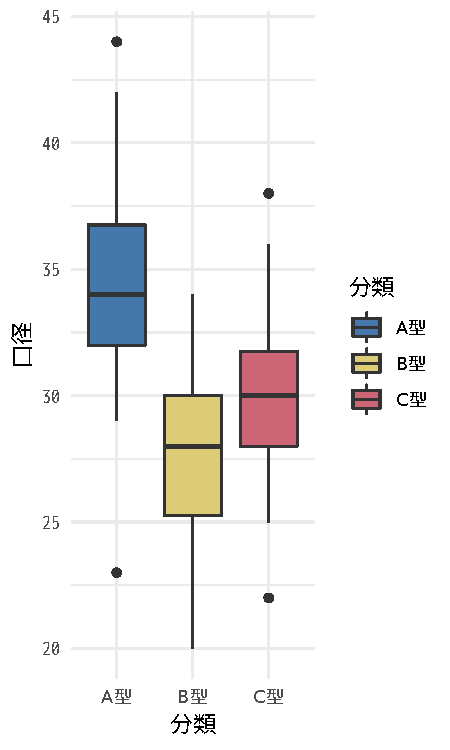
\includegraphics{document_files/figure-latex/unnamed-chunk-6-1.pdf}

密度図や箱ひげ図では分類ごとの差がよくわかります。
散布図では「B型」と「C型」の違いは明確ではありませんでしたが、1変量ずつ比較することで分類ごとの差が明確になりました。。

\subsubsection{まとめ}

\begin{itemize}
\tightlist
\item
  安易な散布図で納得しない。
\item
  連続量の分布を知りたければヒストグラム
\item
  離散量ごとの分布の違いを知りたければ箱ひげ図
\end{itemize}

\subsection{多重比較}

箱ひげ図によって、土器の口径は分類によって差がありそうだということがわかりました。
差があるかどうかを定量的に判断するために統計的な検定を行います。

この場合、3つの群に分類されていますので、3つの群同士に差があるかどうかを統計的に確かめることになります。
多群の差の検定手法の一つである「多重比較」を行います。

\subsubsection{分散分析}

最初に分散分析で品種によって差があるかどうかを確認します。
p値が2.2e-16と極めて小さい値をとることから、品種によって差があることがわかります。

\begin{Shaded}
\begin{Highlighting}[]
\CommentTok{# aov関数の結果をanova関数に渡します。}
\CommentTok{# aov関数の第一引数は連続量~離散量}
\KeywordTok{aov}\NormalTok{(口径}\OperatorTok{~}\NormalTok{分類,}\DataTypeTok{data=}\NormalTok{pot)}\OperatorTok\StringTok{ }\KeywordTok{anova}\NormalTok{()}\OperatorTok\KeywordTok{kable}\NormalTok{(}\DataTypeTok{format=}\StringTok{"markdown"}\NormalTok{)}
\end{Highlighting}
\end{Shaded}

\begin{longtable}[]{@{}lrrrrr@{}}
\toprule
& Df & Sum Sq & Mean Sq & F value & Pr(\textgreater{}F)\tabularnewline
\midrule
\endhead
分類 & 2 & 1134.493 & 567.24667 & 49.16004 & 0\tabularnewline
Residuals & 147 & 1696.200 & 11.53878 & NA & NA\tabularnewline
\bottomrule
\end{longtable}

\hypertarget{tukeyhsd}{%
\subsubsection{TukeyHSD関数で多重比較}\label{tukeyhsd}}

次にどの分類同士で差があるのかを調べるために多重比較を行います。
いずれ分類でも有意な差が確認できます。

\begin{Shaded}
\begin{Highlighting}[]
\CommentTok{# aov関数の結果をTukeyHSD関数に渡す}
\NormalTok{tkh<-}\KeywordTok{aov}\NormalTok{(口径}\OperatorTok{~}\NormalTok{分類,}\DataTypeTok{data=}\NormalTok{pot)}\OperatorTok\KeywordTok{TukeyHSD}\NormalTok{()}
\NormalTok{tkh}\OperatorTok{$}\NormalTok{分類}\OperatorTok\KeywordTok{kable}\NormalTok{(}\DataTypeTok{format=}\StringTok{"markdown"}\NormalTok{)}
\end{Highlighting}
\end{Shaded}

\begin{longtable}[]{@{}lrrrr@{}}
\toprule
& diff & lwr & upr & p adj\tabularnewline
\midrule
\endhead
B型-A型 & -6.58 & -8.1885528 & -4.971447 & 0.0000000\tabularnewline
C型-A型 & -4.54 & -6.1485528 & -2.931447 & 0.0000000\tabularnewline
C型-B型 & 2.04 & 0.4314472 & 3.648553 & 0.0087802\tabularnewline
\bottomrule
\end{longtable}

\hypertarget{-1}{%
\subsubsection{まとめ}\label{-1}}

多重比較は強力な手法ですが、統計的に有意であることが考古学的に有意であることを保証するわけではありません。検定で有意差を証明することは大切ではありますが、必須の作業ではありません。適切な手法でデータの分布を可視化するだけで、多くの場合は十分です。

\subsection{ヒストグラムを活用する}

連続量のデータがあった場合、まず何をするのが適切か?と問われれば、「分布の形を確認する」と答えることになります。
分布の形を可視化する最善の方法はヒストグラムを描くことです。

\subsubsection{刀身長の分布}

北海道恵庭市西島松5遺跡出土の奈良時代の刀剣類のデータを使用します。

\begin{Shaded}
\begin{Highlighting}[]
\NormalTok{iron<-}\KeywordTok{read.csv}\NormalTok{(}\StringTok{"data/iron.csv"}\NormalTok{)}
\NormalTok{iron[,}\KeywordTok{c}\NormalTok{(}\DecValTok{4}\OperatorTok{:}\DecValTok{12}\NormalTok{)]}\OperatorTok\KeywordTok{head}\NormalTok{()}\OperatorTok\KeywordTok{kable}\NormalTok{()}
\end{Highlighting}
\end{Shaded}

\begin{longtable}[]{@{}ccccccccc@{}}
\toprule
全長 & 刀身長 & 茎長 & 刀身先幅 & 刀身元幅 & 刀身元厚 & 茎先幅 & 茎元幅
& 茎先厚\tabularnewline
\midrule
\endhead
6.2 & 4.00 & 2.20 & 0.80 & 1.00 & 0.40 & 0.60 & 0.80 &
0.30\tabularnewline
9.2 & 4.30 & 4.90 & 0.90 & 1.00 & 0.30 & 0.40 & 1.05 &
0.30\tabularnewline
6.9 & 4.70 & 2.20 & 1.00 & 1.10 & 0.25 & 0.65 & 0.80 &
0.20\tabularnewline
8.2 & 6.00 & 2.20 & 0.65 & 0.80 & 0.30 & 0.80 & 1.05 &
0.30\tabularnewline
11.8 & 6.30 & 5.50 & 0.60 & 1.25 & 0.30 & 0.60 & 1.05 &
0.30\tabularnewline
12.0 & 6.44 & 5.56 & 1.40 & 1.90 & 0.40 & 0.65 & 1.25 &
0.34\tabularnewline
\bottomrule
\end{longtable}

私たちには予備知識として、刀剣には刀子のようなマキリ状の小さなもの、刃渡り30cm前後の短刀、刃渡り60cmを超えるような太刀があることを知っていますが、そうした予備知識をいったん忘れてデータを観察します。

\begin{Shaded}
\begin{Highlighting}[]
\NormalTok{p<-iron}\OperatorTok
\StringTok{    }\KeywordTok{ggplot}\NormalTok{(}\KeywordTok{aes}\NormalTok{(}\DataTypeTok{x=}\NormalTok{刀身長))}\OperatorTok{+}
\StringTok{    }\KeywordTok{geom_histogram}\NormalTok{()}\OperatorTok{+}
\StringTok{    }\KeywordTok{theme_minimal}\NormalTok{()}
\KeywordTok{print}\NormalTok{(p)}
\end{Highlighting}
\end{Shaded}

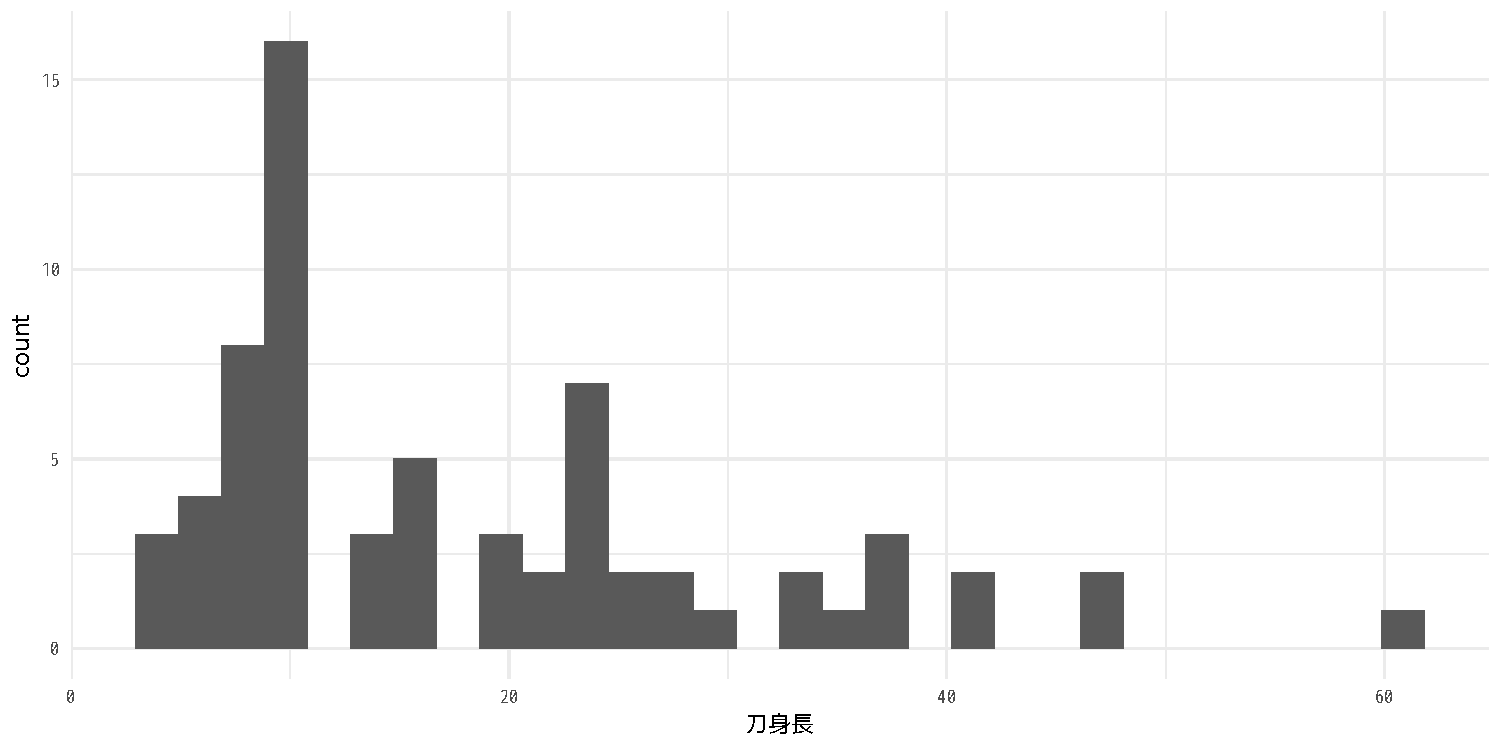
\includegraphics{document_files/figure-latex/unnamed-chunk-10-1.pdf}

刀身長の分布は10cm、20cm超、40cm前後に峰をもつ3峰分布といえるでしょうか?私たちの予備知識に照らし合わせると、刀子、短刀、短めの太刀に相当する刀身サイズの分化があると推測できます。
ここではこれ以上踏み込みませんが、「分布の形はヒストグラム」というのが鉄則です。

\subsubsection{散布図ではだめなのか?}

2変量が用意できる場合は散布図で比較することも可能と思われるかもしれません。
実際に考古学の論文や発掘調査報告書では、分布の可視化に散布図を用いているケースが非常に多いと感じます。

下の図は、刀身長と刀身元幅の散布図です。
この図が間違いとは言いませんが、ヒストグラムと比較して、分布の形がわかりやすいと言えるでしょうか?
下の散布図から分布に関して何らかの結論を出すのは難しいのではないでしょうか。

\begin{Shaded}
\begin{Highlighting}[]
\NormalTok{p<-iron}\OperatorTok
\StringTok{    }\KeywordTok{ggplot}\NormalTok{(}\KeywordTok{aes}\NormalTok{(}\DataTypeTok{x=}\NormalTok{刀身長,}\DataTypeTok{y=}\NormalTok{刀身元幅))}\OperatorTok{+}
\StringTok{    }\KeywordTok{geom_point}\NormalTok{()}\OperatorTok{+}
\StringTok{    }\KeywordTok{theme_minimal}\NormalTok{()}
\KeywordTok{print}\NormalTok{(p)}
\end{Highlighting}
\end{Shaded}

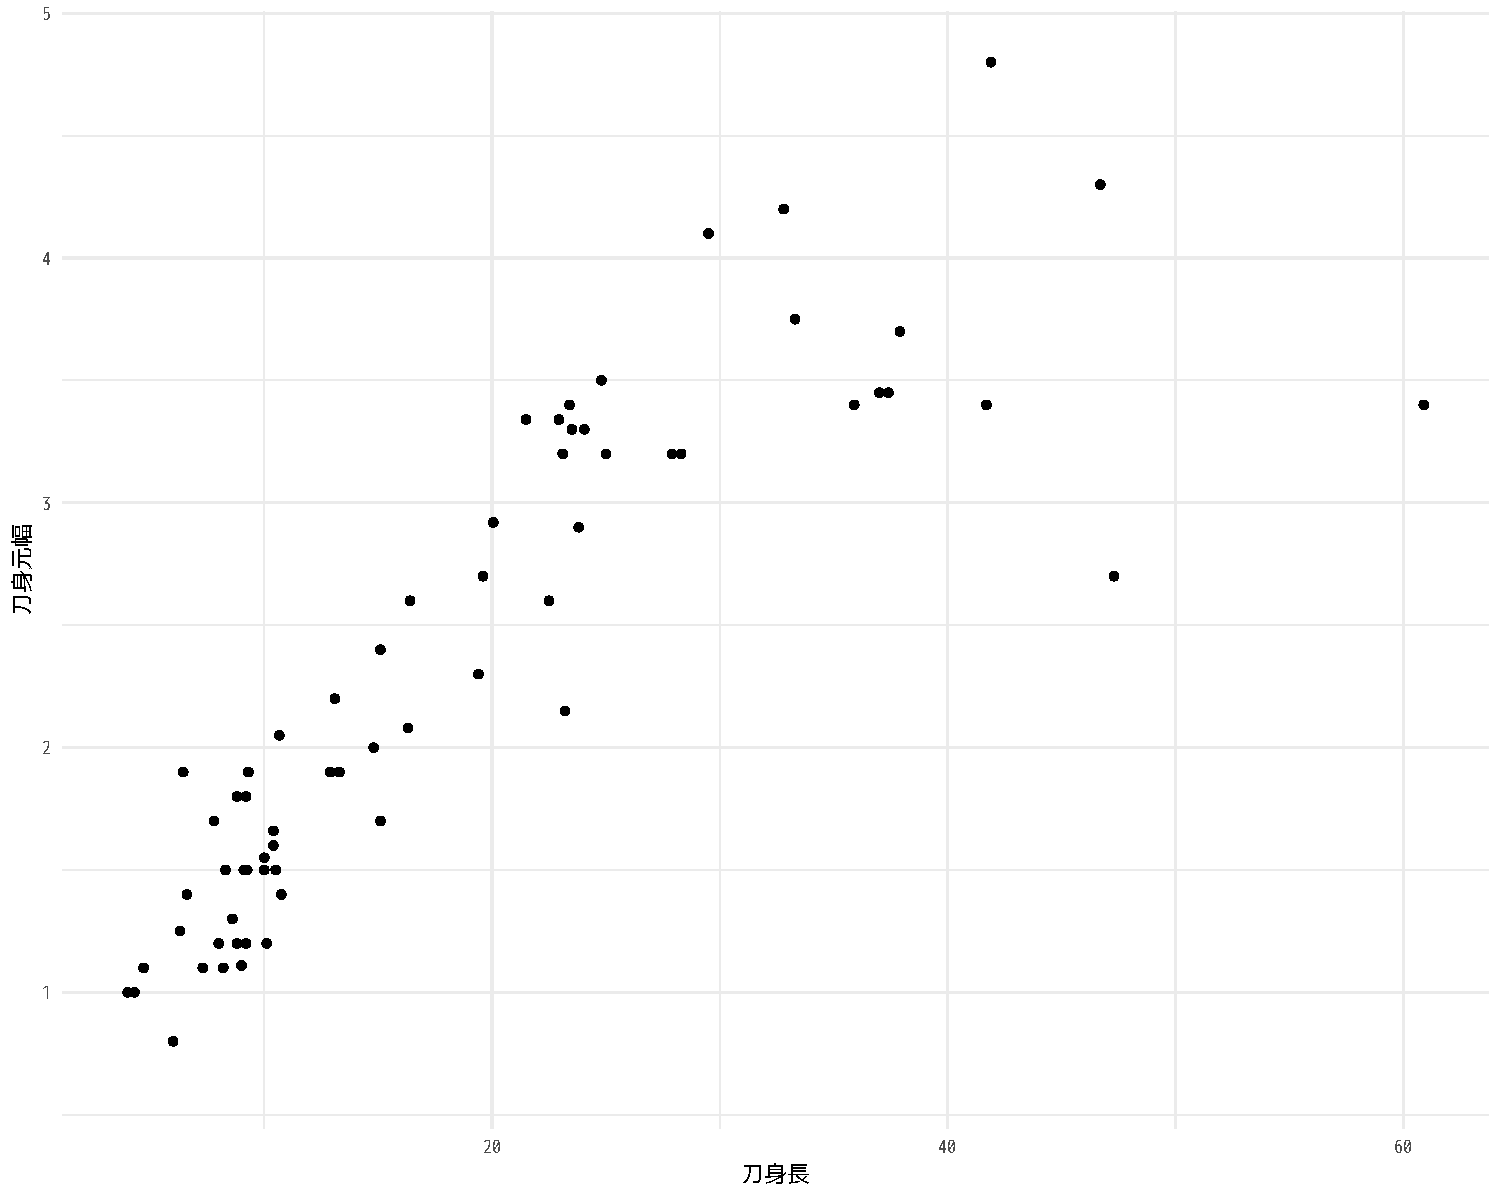
\includegraphics{document_files/figure-latex/unnamed-chunk-11-1.pdf}

\subsubsection{ヒストグラムを使うべき理由}

ヒストグラムのもう一つの利点は、分布の形状を数的モデルに近似して比較できることです。
下の図は正規曲線を重ねた刀身長のヒストグラムです。
正規化しているので、Y軸は密度になっていますが、分布の形は変化しません。

\begin{Shaded}
\begin{Highlighting}[]
\CommentTok{# 正規曲線作成のための統計量}
\NormalTok{iron}\OperatorTok
\StringTok{    }\KeywordTok{summarise}\NormalTok{(}\DataTypeTok{mean=}\KeywordTok{mean}\NormalTok{(刀身長,}\DataTypeTok{na.rm=}\NormalTok{T),}\DataTypeTok{sd=}\KeywordTok{sd}\NormalTok{(刀身長,}\DataTypeTok{na.rm=}\NormalTok{T))}\OperatorTok
\StringTok{    }\KeywordTok{kable}\NormalTok{()}
\end{Highlighting}
\end{Shaded}

\begin{longtable}[]{@{}rr@{}}
\toprule
mean & sd\tabularnewline
\midrule
\endhead
18.4003 & 12.49029\tabularnewline
\bottomrule
\end{longtable}

\begin{Shaded}
\begin{Highlighting}[]
\CommentTok{# 正規曲線作成}
\NormalTok{x<-}\KeywordTok{seq}\NormalTok{(}\DecValTok{0}\NormalTok{, }\DecValTok{60}\NormalTok{, }\FloatTok{0.1}\NormalTok{)}
\NormalTok{nom <-}\StringTok{ }\NormalTok{x}\OperatorTok\KeywordTok{dnorm}\NormalTok{(}\DataTypeTok{mean=}\FloatTok{18.40}\NormalTok{, }\DataTypeTok{sd=}\FloatTok{12.49}\NormalTok{)}
\NormalTok{nom2<-}\KeywordTok{data.frame}\NormalTok{(}\DataTypeTok{X=}\NormalTok{x,}\DataTypeTok{Y=}\NormalTok{nom)}
\CommentTok{#正規曲線付きヒストグラム}
\NormalTok{p<-iron}\OperatorTok
\StringTok{    }\KeywordTok{ggplot}\NormalTok{(}\KeywordTok{aes}\NormalTok{(}\DataTypeTok{x=}\NormalTok{刀身長,}\DataTypeTok{y=}\NormalTok{..density..))}\OperatorTok{+}
\StringTok{        }\KeywordTok{geom_histogram}\NormalTok{()}\OperatorTok{+}
\StringTok{        }\KeywordTok{geom_line}\NormalTok{(}\DataTypeTok{data=}\NormalTok{nom2,}\KeywordTok{aes}\NormalTok{(}\DataTypeTok{x=}\NormalTok{x,}\DataTypeTok{y=}\NormalTok{Y))}\OperatorTok{+}
\StringTok{        }\KeywordTok{scale_colour_ptol}\NormalTok{()}\OperatorTok{+}
\StringTok{        }\KeywordTok{theme_minimal}\NormalTok{()}
\KeywordTok{print}\NormalTok{(p)}
\end{Highlighting}
\end{Shaded}

\begin{verbatim}
## `stat_bin()` using `bins = 30`. Pick better value with `binwidth`.
\end{verbatim}

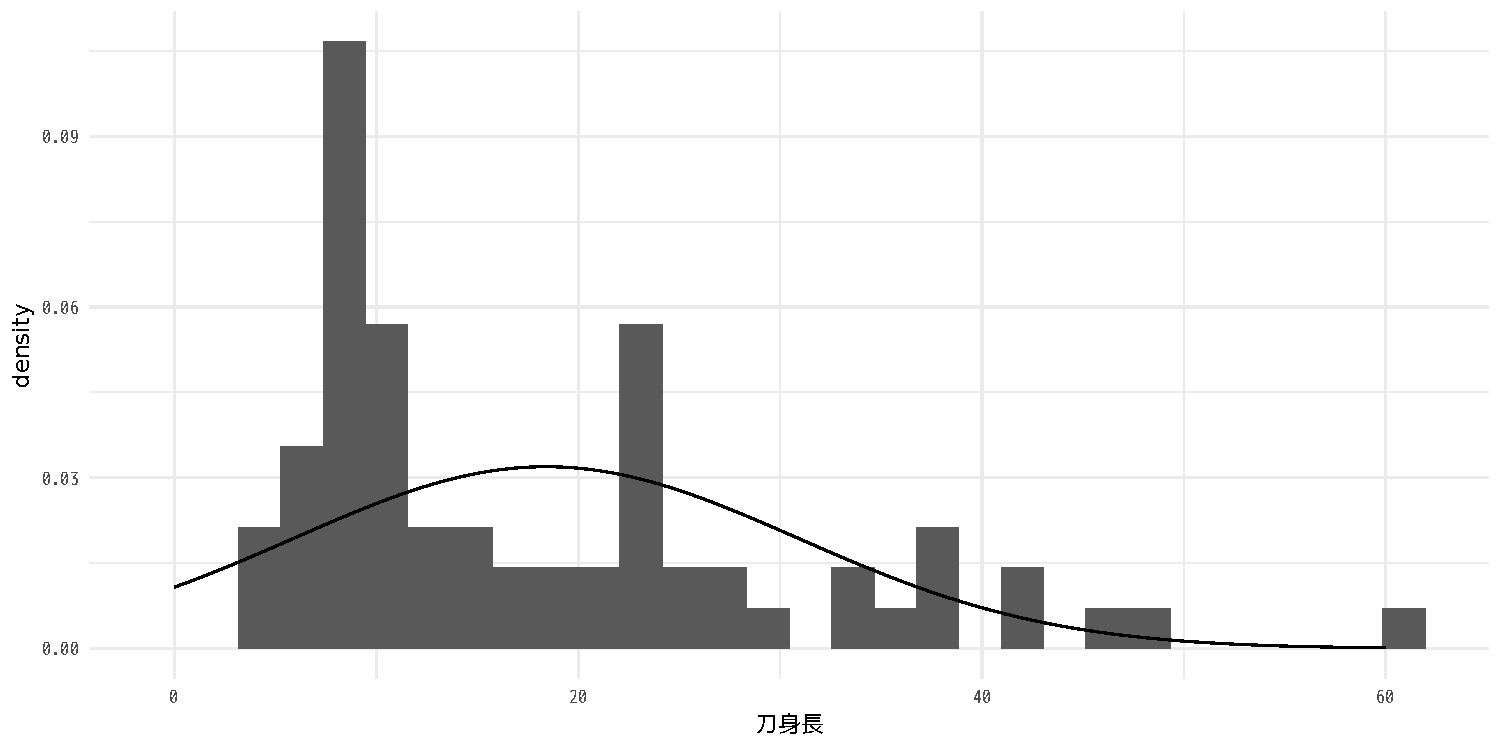
\includegraphics{document_files/figure-latex/unnamed-chunk-13-1.pdf}

刀身長のヒストグラムと正規分布曲線を重ねることによって、刀身長の分布が正規分布から大きく外れていることがはっきりします。
これは、散布図では絶対に表現できません。
上記のヒストグラムから、古代の刀剣に複数のサイズ規範があることは確信できそうです。

\subsubsection{なぜヒストグラムは使われないのだろうか?}

理由の一つとして、ヒストグラムのもつ「数的モデルとの近似が容易である」という特性を考古学の研究者が活かせていない、ということが考えられます。
正規分布とは何か、正規分布で近似できるということはどのような意味をもつのか、そのような判断が難しいのだろうと思います。

\subsubsection{エクセルでヒストグラム}

もう一つの大きな理由は「エクセルでヒストグラムを作りにくい」ということかもしれません。
エクセルでヒストグラムを作れないわけではないのですが、度数分布表から棒グラフとして作成することになるので、一手間かかります。

ビン幅の調整をするにも、いちいち度数分布表を作り直さないといけない、ということも面倒です。
こうした理由でヒストグラムが敬遠されるではないかと感じています。

\subsection{構成比のグラフ表現}

北海道内近世後期の遺跡出土の陶磁器組成のデータを用いて構成比のグラフ表現について考えます。

\begin{Shaded}
\begin{Highlighting}[]
\CommentTok{# データ読み込み}
\NormalTok{toj<-}\KeywordTok{read.csv}\NormalTok{(}\StringTok{"data/pot.csv"}\NormalTok{)}
\CommentTok{# データの順序定義}
\NormalTok{toj}\OperatorTok{$}\NormalTok{器種<-toj}\OperatorTok{$}\NormalTok{器種}\OperatorTok
\StringTok{    }\KeywordTok{factor}\NormalTok{(}\DataTypeTok{levels=}\KeywordTok{c}\NormalTok{(}\StringTok{"碗"}\NormalTok{,}\StringTok{"皿"}\NormalTok{,}\StringTok{"その他食膳具"}\NormalTok{,}\StringTok{"壺・甕・瓶"}\NormalTok{,}
        \StringTok{"土瓶"}\NormalTok{,}\StringTok{"鍋"}\NormalTok{,}\StringTok{"すり鉢"}\NormalTok{,}\StringTok{"灯明皿・油注"}\NormalTok{,}\StringTok{"その他"}\NormalTok{))}
\NormalTok{toj}\OperatorTok\KeywordTok{head}\NormalTok{()}\OperatorTok\KeywordTok{kable}\NormalTok{()}
\end{Highlighting}
\end{Shaded}

\begin{longtable}[]{@{}llc@{}}
\toprule
遺跡名 & 器種 & 点数\tabularnewline
\midrule
\endhead
弁天貝塚 & 碗 & 134\tabularnewline
弁天貝塚 & 皿 & 84\tabularnewline
弁天貝塚 & その他食膳具 & 34\tabularnewline
弁天貝塚 & 土瓶 & 6\tabularnewline
弁天貝塚 & 鍋 & 0\tabularnewline
弁天貝塚 & すり鉢 & 46\tabularnewline
\bottomrule
\end{longtable}

棒グラフは離散量を表現するために使われます。遺跡ごとあるいは住居跡ごとに出土遺物の構成比を調べる際に使用する可視化手法を紹介します。もっとも大切なことは、\textbf{円グラフを使わない}ということです。

人間の目は線の長さや点の位置を把握することには長けていますが、面積の大小を認識するのは苦手です。
円グラフは面積で比率を表すので比率の比較には向いていないのです。

\begin{Shaded}
\begin{Highlighting}[]
\NormalTok{toj_pie<-toj}\OperatorTok\KeywordTok{group_by}\NormalTok{(器種)}\OperatorTok\KeywordTok{summarise}\NormalTok{(点数=}\KeywordTok{sum}\NormalTok{(点数))}
\KeywordTok{pie}\NormalTok{(toj_pie}\OperatorTok{$}\NormalTok{点数,}\DataTypeTok{labels=}\NormalTok{toj_pie}\OperatorTok{$}\NormalTok{器種)}
\end{Highlighting}
\end{Shaded}

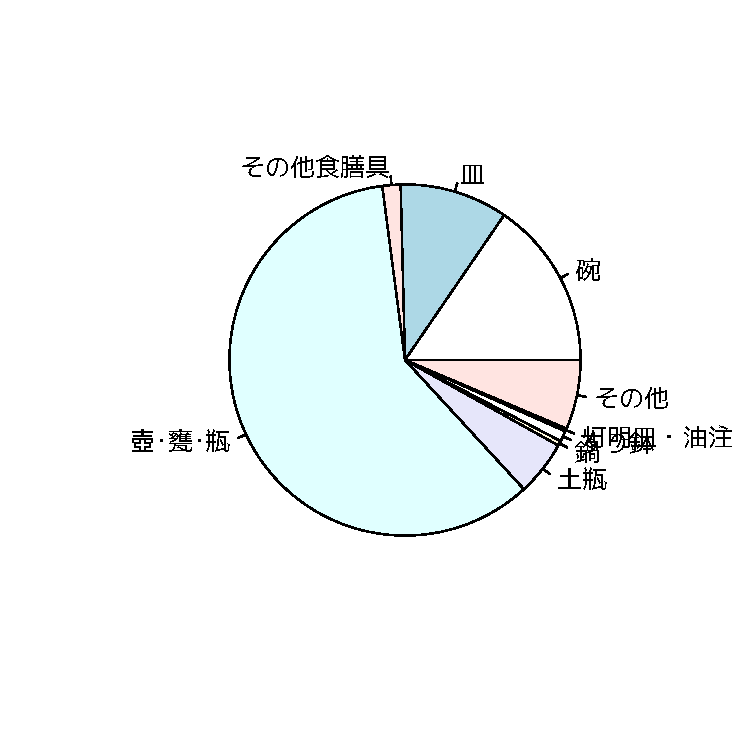
\includegraphics{document_files/figure-latex/unnamed-chunk-15-1.pdf}

特に3D円グラフは目の錯覚を利用して、特定の値を大きく(小さく)見せるための手法です。公文書や学術的な報告では\textbf{絶対に}使うべきものではありません。

なお、Rで円グラフ(Pie
charts)のヘルプを表示すると次のように記載されています。

Note:

\begin{verbatim}
 Pie charts are a very bad way of displaying information.  The eye
 is good at judging linear measures and bad at judging relative
 areas.  A bar chart or dot chart is a preferable way of displaying
 this type of data.

 Cleveland (1985), page 264: “Data that can be shown by pie charts
 always can be shown by a dot chart.  This means that judgements of
 position along a common scale can be made instead of the less
 accurate angle judgements.” This statement is based on the
 empirical investigations of Cleveland and McGill as well as
 investigations by perceptual psychologists.
\end{verbatim}

意訳

円グラフは不適切な可視化手法です。人間の目は直線的な形状の判断には優れていますが、面の比較は苦手です。円グラフで表現できるデータは棒グラフやドットチャートで表現するべきです。

「円グラフで表示できるデータは全てドットチャートで表現できます。円の内角による不正確な判断ではなく、誰もが判断できるモノサシを用いるべきであることを意味しています」(Cleveland
1985,p264)

\subsection{構成比棒グラフ}

構成比を比較するために使われるのが構成比棒グラフです。長さや位置によって視覚化されるため、正確な読み取りが可能です。
構成比棒グラフは比率を比較するには非常に優れたグラフ表現です。

\begin{Shaded}
\begin{Highlighting}[]
\NormalTok{p<-toj}\OperatorTok
\StringTok{    }\KeywordTok{ggplot}\NormalTok{(}\KeywordTok{aes}\NormalTok{(}\DataTypeTok{x=}\NormalTok{遺跡名,}\DataTypeTok{y=}\NormalTok{点数,}\DataTypeTok{fill=}\NormalTok{器種))}\OperatorTok{+}
\StringTok{        }\KeywordTok{geom_bar}\NormalTok{(}\DataTypeTok{stat=}\StringTok{"identity"}\NormalTok{,}\DataTypeTok{position=}\StringTok{"fill"}\NormalTok{)}\OperatorTok{+}
\StringTok{        }\KeywordTok{coord_flip}\NormalTok{()}\OperatorTok{+}
\StringTok{        }\KeywordTok{scale_fill_ptol}\NormalTok{()}\OperatorTok{+}
\StringTok{        }\KeywordTok{theme_minimal}\NormalTok{()}
\KeywordTok{print}\NormalTok{(p)}
\end{Highlighting}
\end{Shaded}

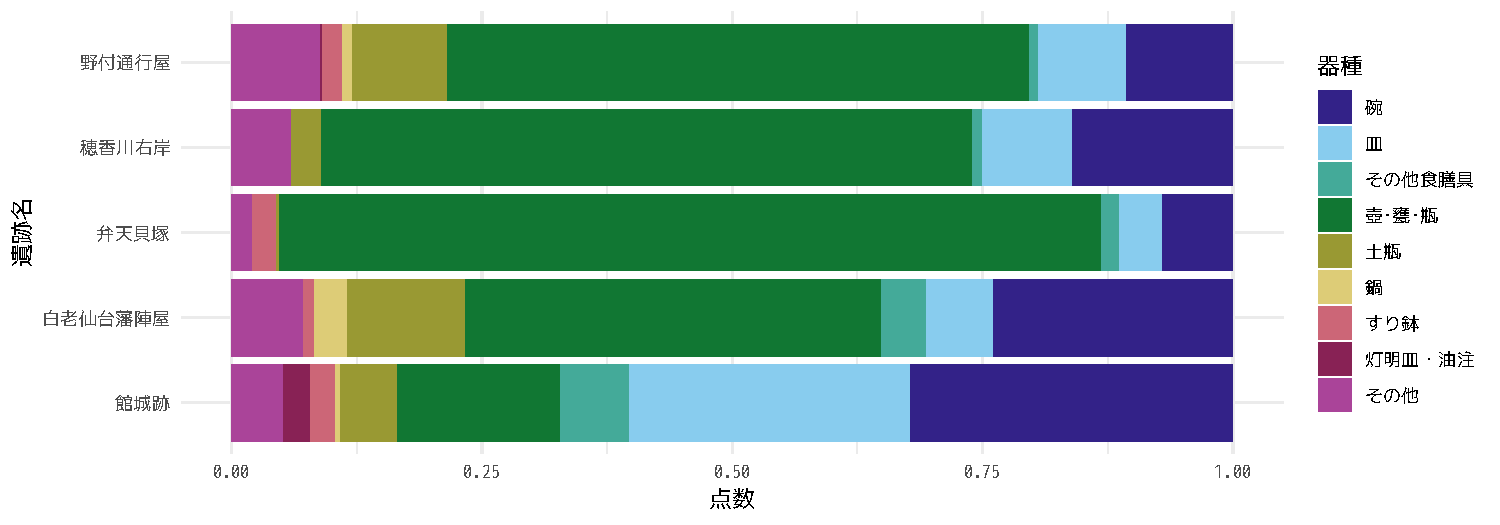
\includegraphics{document_files/figure-latex/unnamed-chunk-16-1.pdf}

ただし、発掘調査報告書でカラーグラフが掲載できるケースは稀で、大半はグレースケールで表現されることになります。
下のグラフはモニター上ではなんとか識別できますが、オフセット印刷の仕上がりでこれを識別することは不可能です。
凡例との対比は特に困難です。

オフセット印刷の場合、グレスケール(網掛け)は20〜30\%スパンが識別できるぎりぎりなので、構成比では4群〜5群が限界となります。

\begin{Shaded}
\begin{Highlighting}[]
\NormalTok{p<-toj}\OperatorTok
\StringTok{    }\KeywordTok{ggplot}\NormalTok{(}\KeywordTok{aes}\NormalTok{(}\DataTypeTok{x=}\NormalTok{遺跡名,}\DataTypeTok{y=}\NormalTok{点数,}\DataTypeTok{fill=}\NormalTok{器種))}\OperatorTok{+}
\StringTok{        }\KeywordTok{geom_bar}\NormalTok{(}\DataTypeTok{stat=}\StringTok{"identity"}\NormalTok{,}\DataTypeTok{position=}\StringTok{"fill"}\NormalTok{)}\OperatorTok{+}
\StringTok{        }\KeywordTok{coord_flip}\NormalTok{()}\OperatorTok{+}
\StringTok{        }\KeywordTok{scale_fill_brewer}\NormalTok{(}\DataTypeTok{palette=}\StringTok{"Greys"}\NormalTok{)}\OperatorTok{+}
\StringTok{        }\KeywordTok{theme_minimal}\NormalTok{()}
\KeywordTok{print}\NormalTok{(p)}
\end{Highlighting}
\end{Shaded}

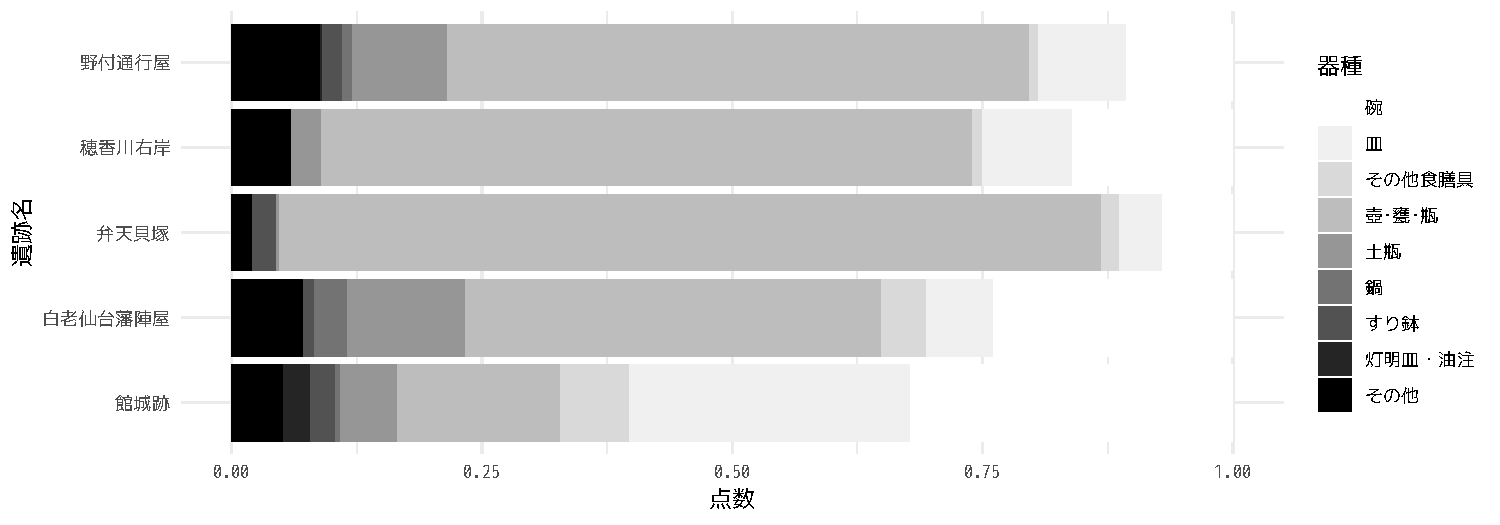
\includegraphics{document_files/figure-latex/unnamed-chunk-17-1.pdf}

\hypertarget{1}{%
\subsubsection{解決法1 カテゴリーを減らす}\label{1}}

グラフ表現は複雑な現実をシンプルに割り切って視覚的に表現するためのものです。カテゴリー群が多すぎて識別が困難ならば、カテゴリーを減らすことをまず考えるべきです。
3群まで減らせばオフセット印刷でも対応可能なグレースケールのグラフになります。

\begin{Shaded}
\begin{Highlighting}[]
\CommentTok{# 食膳具、貯蔵具、その他に区分}
\NormalTok{toj2<-toj}\OperatorTok
\StringTok{    }\KeywordTok{mutate}\NormalTok{(大別器種 =}\StringTok{ }\KeywordTok{case_when}\NormalTok{(}
        \KeywordTok{grepl}\NormalTok{(}\StringTok{"碗"}\NormalTok{,器種)}\OperatorTok{|}\KeywordTok{grepl}\NormalTok{(}\StringTok{"皿"}\NormalTok{,器種)}\OperatorTok{|}\KeywordTok{grepl}\NormalTok{(}\StringTok{"その他の食膳具"}\NormalTok{,器種)  }\OperatorTok{==}\StringTok{ }\OtherTok{TRUE} \OperatorTok{~}\StringTok{ "食膳具"}\NormalTok{,}
        \KeywordTok{grepl}\NormalTok{(}\StringTok{"壺・甕・瓶"}\NormalTok{,器種) }\OperatorTok{==}\StringTok{ }\OtherTok{TRUE} \OperatorTok{~}\StringTok{ "貯蔵具"}\NormalTok{,}
        \KeywordTok{grepl}\NormalTok{(}\StringTok{"灯明皿・油注"}\NormalTok{,器種)}\OperatorTok{|}\KeywordTok{grepl}\NormalTok{(}\StringTok{"その他"}\NormalTok{,器種)}\OperatorTok{|}\KeywordTok{grepl}\NormalTok{(}\StringTok{"すり鉢"}\NormalTok{,器種)}\OperatorTok{|}
\StringTok{            }\KeywordTok{grepl}\NormalTok{(}\StringTok{"鍋"}\NormalTok{,器種)}\OperatorTok{|}\KeywordTok{grepl}\NormalTok{(}\StringTok{"土瓶"}\NormalTok{,器種) }\OperatorTok{==}\StringTok{ }\OtherTok{TRUE} \OperatorTok{~}\StringTok{ "その他"}\NormalTok{,}
\NormalTok{        ))}
\CommentTok{# 3区分の構成比棒グラフ}
\NormalTok{p<-toj2}\OperatorTok
\StringTok{    }\KeywordTok{ggplot}\NormalTok{(}\KeywordTok{aes}\NormalTok{(}\DataTypeTok{x=}\NormalTok{遺跡名,}\DataTypeTok{y=}\NormalTok{点数,}\DataTypeTok{fill=}\NormalTok{大別器種))}\OperatorTok{+}
\StringTok{        }\KeywordTok{geom_bar}\NormalTok{(}\DataTypeTok{stat=}\StringTok{"identity"}\NormalTok{,}\DataTypeTok{position=}\StringTok{"fill"}\NormalTok{)}\OperatorTok{+}
\StringTok{        }\KeywordTok{coord_flip}\NormalTok{()}\OperatorTok{+}
\StringTok{        }\KeywordTok{scale_fill_brewer}\NormalTok{(}\DataTypeTok{palette=}\StringTok{"Greys"}\NormalTok{)}\OperatorTok{+}
\StringTok{        }\KeywordTok{theme_minimal}\NormalTok{()}
\KeywordTok{print}\NormalTok{(p)}
\end{Highlighting}
\end{Shaded}

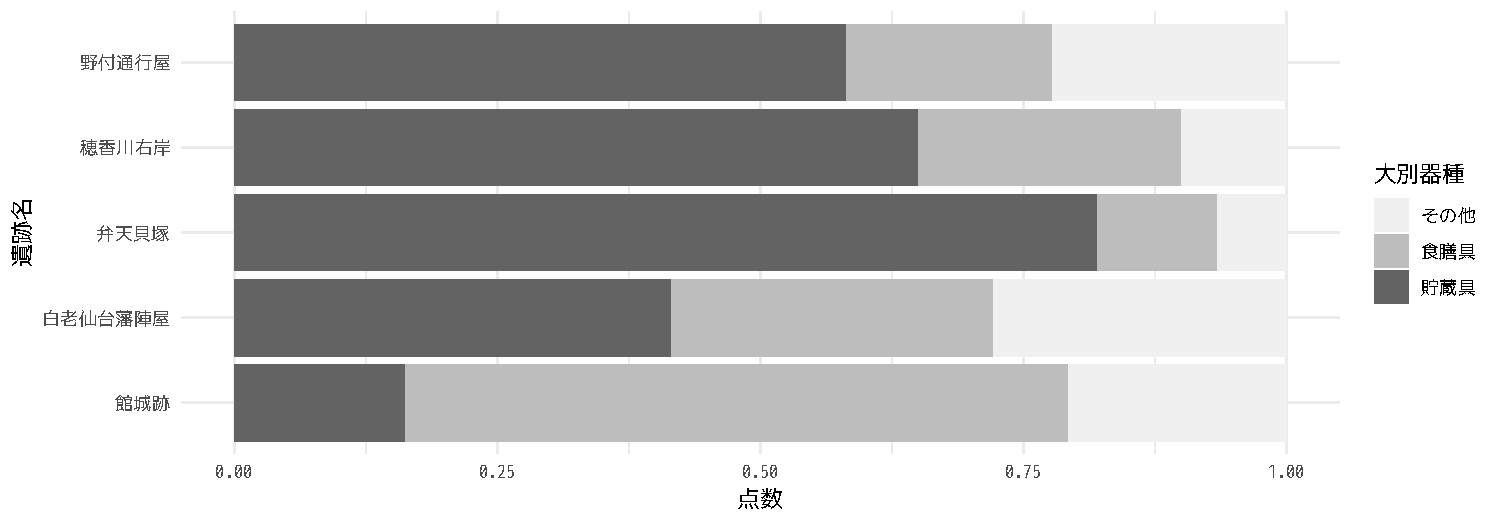
\includegraphics{document_files/figure-latex/unnamed-chunk-18-1.pdf}

\hypertarget{2}{%
\subsubsection{解決法2 ファセットされた棒グラフを使う}\label{2}}

どうしてもカテゴリー数を減らしたくない場合は、群変数を器種にとって遺跡ごとにファセットします。花粉分析などの分析結果でよく見る形のグラフです。よほどカテゴリーが多くない限り、表現として成立していますし、オフセット印刷原稿としても対応可能です。

\begin{Shaded}
\begin{Highlighting}[]
\NormalTok{p<-toj}\OperatorTok
\StringTok{    }\KeywordTok{ggplot}\NormalTok{(}\KeywordTok{aes}\NormalTok{(}\DataTypeTok{x=}\NormalTok{器種,}\DataTypeTok{y=}\NormalTok{点数))}\OperatorTok{+}
\StringTok{    }\KeywordTok{geom_bar}\NormalTok{(}\DataTypeTok{stat=}\StringTok{"identity"}\NormalTok{)}\OperatorTok{+}
\StringTok{    }\KeywordTok{coord_flip}\NormalTok{()}\OperatorTok{+}\KeywordTok{facet_wrap}\NormalTok{(}\OperatorTok{~}\NormalTok{遺跡名,}\DataTypeTok{scales=}\StringTok{"free"}\NormalTok{)}\OperatorTok{+}
\StringTok{    }\KeywordTok{theme_minimal}\NormalTok{()}
\KeywordTok{print}\NormalTok{(p)}
\end{Highlighting}
\end{Shaded}

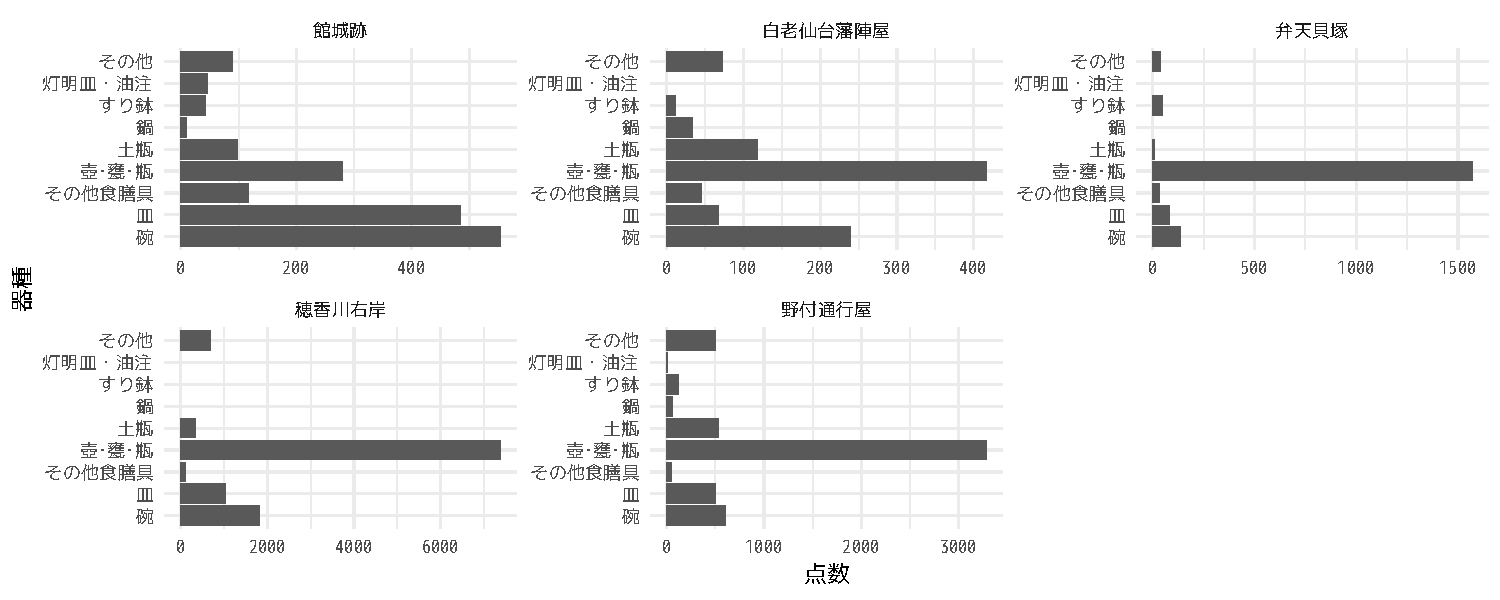
\includegraphics{document_files/figure-latex/unnamed-chunk-19-1.pdf}

\subsection{散布図}

散布図は連続量×連続量の組み合わせのデータで用いられます。考古学の論文・報文でもっとも多く使われるグラフ表現かもしれません。
しかし、散布図が最も得意とする「二変量の関係を可視化する」という用途に使われることが案外少ないように思います。

ヒストグラムの項で用いた土器のデータを使用します。
分析の目的は、口径と器高の関係を調べることです。

\begin{Shaded}
\begin{Highlighting}[]
\NormalTok{p<-pot}\OperatorTok
\StringTok{    }\KeywordTok{ggplot}\NormalTok{(}\KeywordTok{aes}\NormalTok{(}\DataTypeTok{x=}\NormalTok{口径,}\DataTypeTok{y=}\NormalTok{器高))}\OperatorTok{+}
\StringTok{        }\KeywordTok{geom_point}\NormalTok{()}\OperatorTok{+}
\StringTok{        }\KeywordTok{theme_minimal}\NormalTok{()}
\KeywordTok{plot}\NormalTok{(p)}
\end{Highlighting}
\end{Shaded}

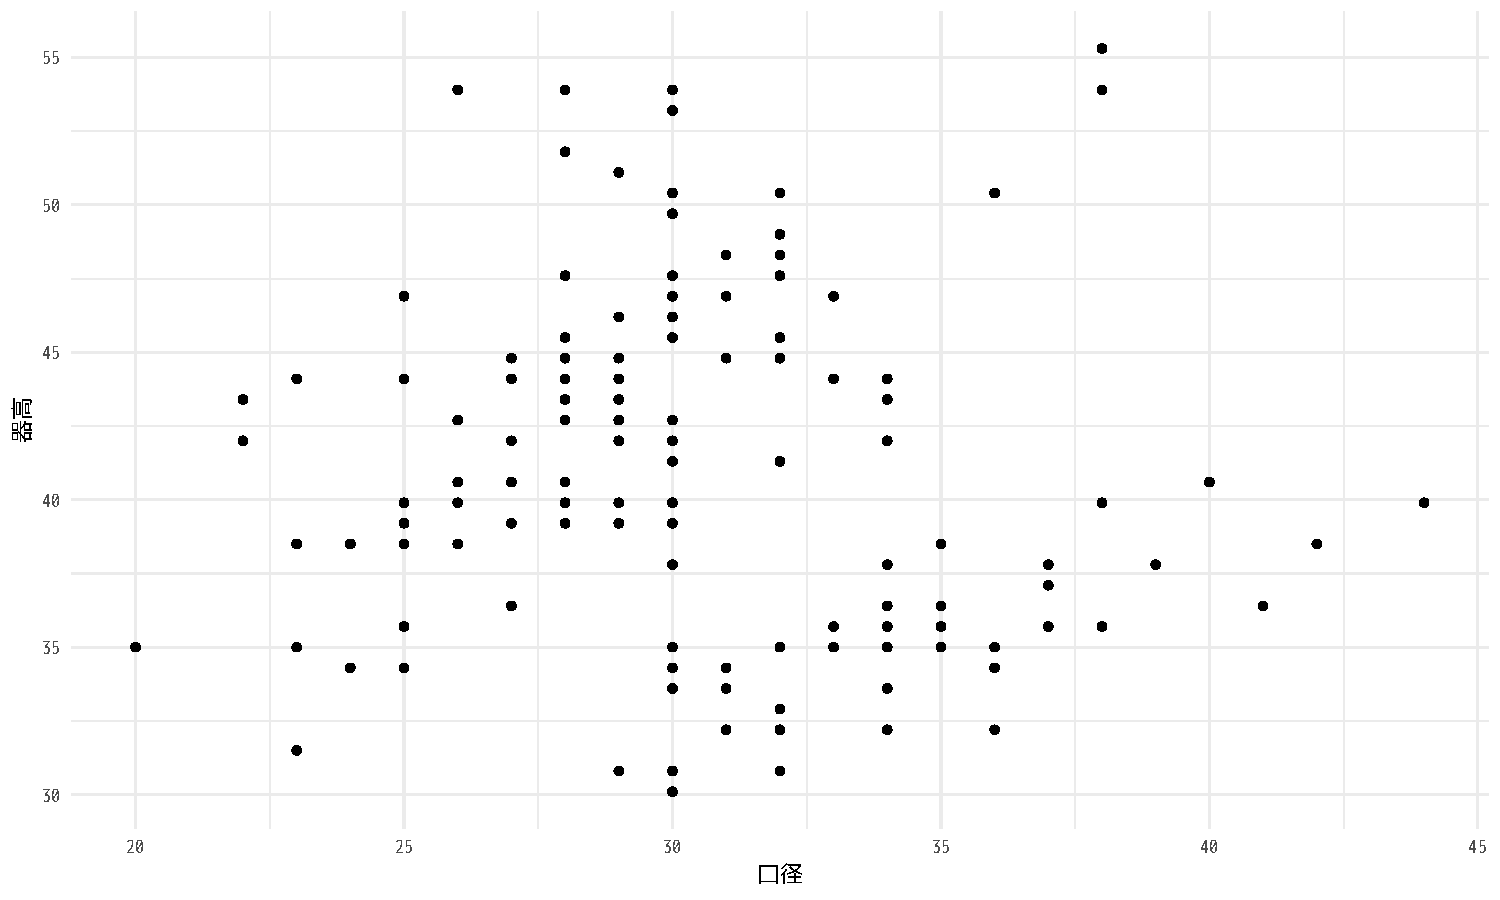
\includegraphics{document_files/figure-latex/unnamed-chunk-20-1.pdf}

土器の分類によって口径と器高が異なると予想されるため、分類群ごとに調べた方が良さそうです。

\begin{Shaded}
\begin{Highlighting}[]
\CommentTok{# 同じグラフに描画}
\NormalTok{p<-pot}\OperatorTok
\StringTok{    }\KeywordTok{ggplot}\NormalTok{(}\KeywordTok{aes}\NormalTok{(}\DataTypeTok{x=}\NormalTok{口径,}\DataTypeTok{y=}\NormalTok{器高,}\DataTypeTok{colour=}\NormalTok{分類))}\OperatorTok{+}
\StringTok{        }\KeywordTok{geom_point}\NormalTok{()}\OperatorTok{+}
\StringTok{        }\KeywordTok{scale_colour_ptol}\NormalTok{()}\OperatorTok{+}
\StringTok{        }\KeywordTok{theme_minimal}\NormalTok{()}
\KeywordTok{plot}\NormalTok{(p)}
\end{Highlighting}
\end{Shaded}

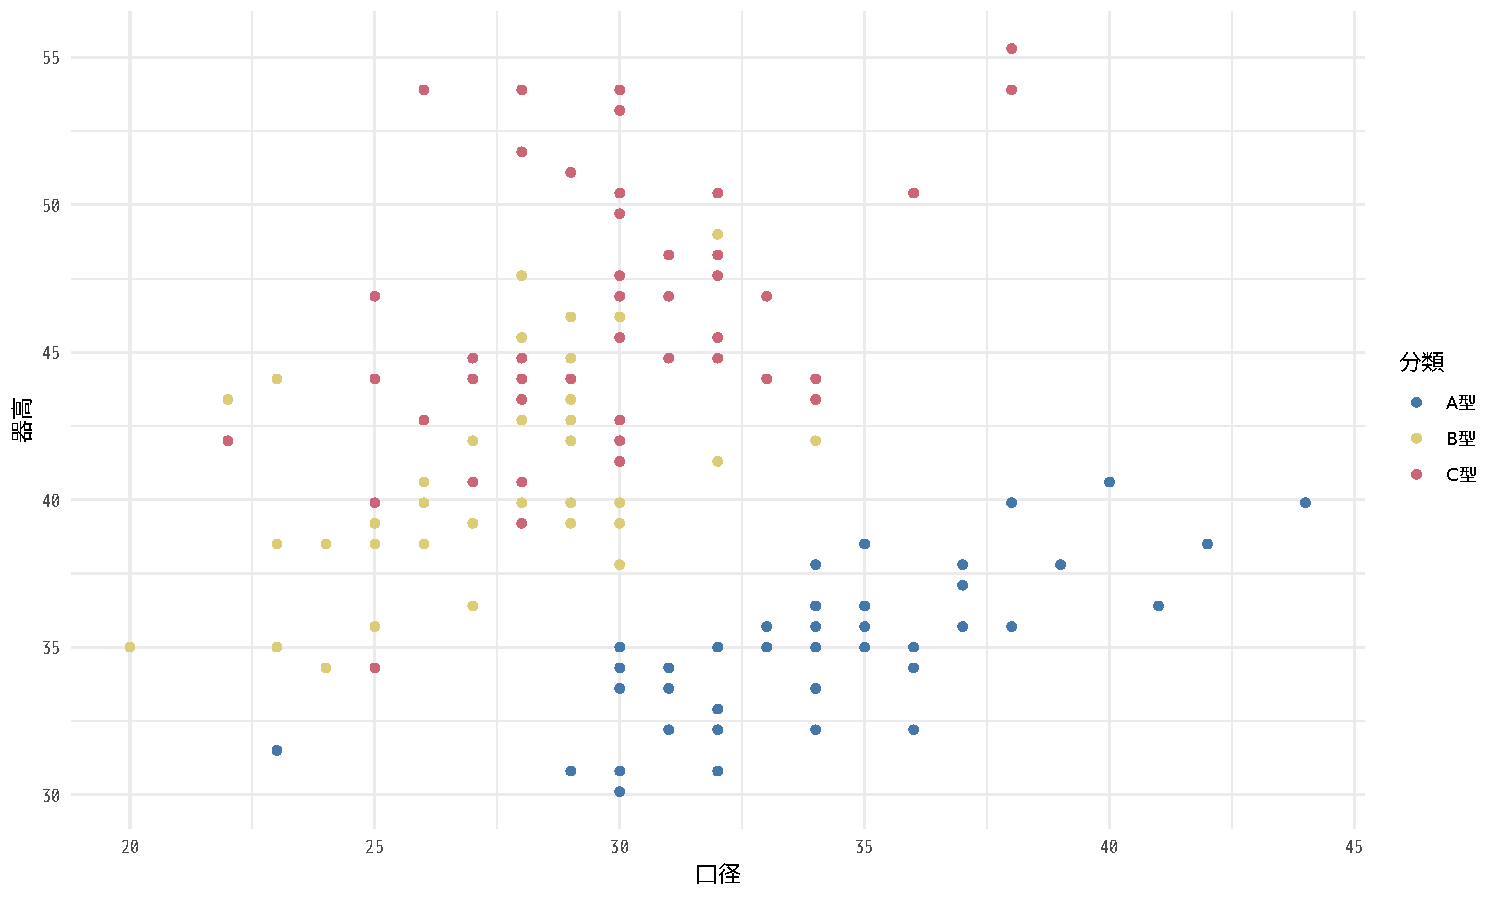
\includegraphics{document_files/figure-latex/unnamed-chunk-21-1.pdf}

\begin{Shaded}
\begin{Highlighting}[]
\CommentTok{# 分類群ごとにファセットして描画}
\NormalTok{p<-pot}\OperatorTok
\StringTok{    }\KeywordTok{ggplot}\NormalTok{(}\KeywordTok{aes}\NormalTok{(}\DataTypeTok{x=}\NormalTok{口径,}\DataTypeTok{y=}\NormalTok{器高,}\DataTypeTok{colour=}\NormalTok{分類))}\OperatorTok{+}
\StringTok{        }\KeywordTok{geom_point}\NormalTok{()}\OperatorTok{+}
\StringTok{        }\KeywordTok{facet_wrap}\NormalTok{(}\OperatorTok{~}\NormalTok{分類,}\DataTypeTok{scales=}\StringTok{"free"}\NormalTok{)}\OperatorTok{+}
\StringTok{        }\KeywordTok{scale_colour_ptol}\NormalTok{()}\OperatorTok{+}
\StringTok{        }\KeywordTok{theme_minimal}\NormalTok{()}
\KeywordTok{plot}\NormalTok{(p)}
\end{Highlighting}
\end{Shaded}

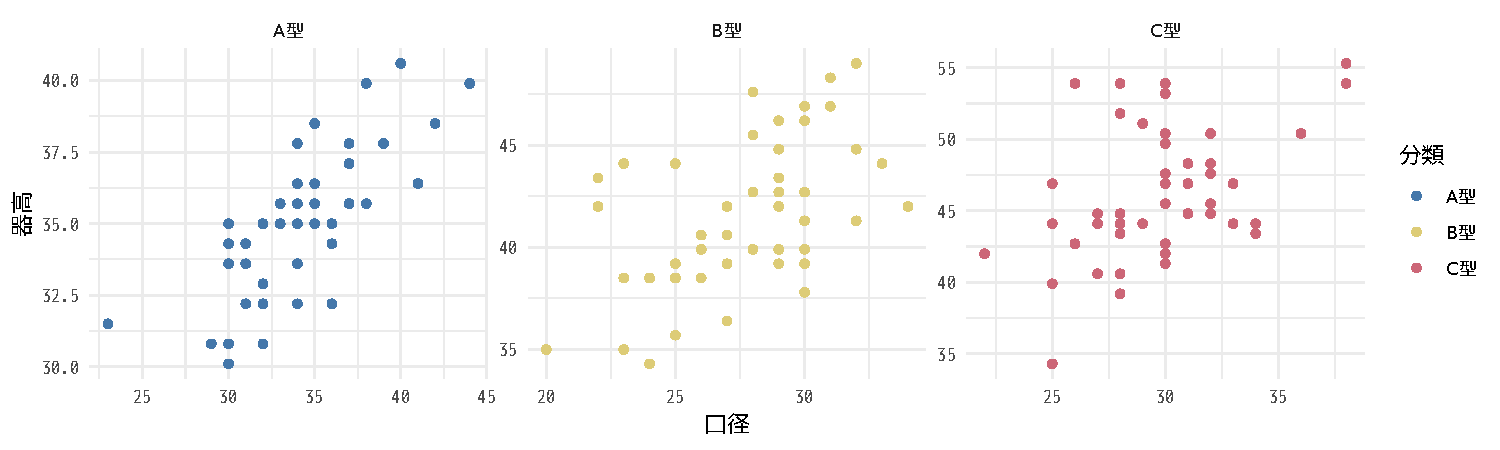
\includegraphics{document_files/figure-latex/unnamed-chunk-22-1.pdf}

散布図を描く場合に同一の領域に色やシェープを変えて描画する場合が多いように感じます。
もちろん間違いではありませんが、「二変量の関係を可視化する」という目的では群ごとにファセットする方が特徴を明確に捉えることができます。
特に発掘調査報告書や雑誌掲載原稿ではカラー図版を使えないケースが多いと思いますので、群ごとにファセットしたほうが読み取りやすいグラフ表現になります。

\subsection{「2変量の関係」とは?}

散布図の評価が難しいのは、「2変量の関係」を何らかの数学的なモデルに近似して表現しなければならないからです。
日頃から数式に慣れている研究者ならともかく、私たち考古学研究者は数学的な訓練をあまり受けていません。
そうしたことから、

\begin{enumerate}
\def\labelenumi{\arabic{enumi}.}
\tightlist
\item
  散布図
\item
  二変量の関係の読み解き
\item
  モデル式の当てはめ 
\end{enumerate}

という手順を踏んで統計処理を進めていないケースが多いように感じています。

\subsubsection{「2変量の関係」を記述する}

まず、考えるべきことは\textbf{2変量の関係が1次式に当てはまるか否か}ということです。

二変量の関係を考えるとき、少し統計に詳しい方は「相関係数」を算出しようと考えると思います。
しかし、相関係数は2変量の関係を1次式をモデルとして1次式との一致度合いを計るものです。
2変量の関係が2次式や反比例式で近似できる場合にはあてはまりません。

\subsubsection{散布図を読み解く}

あらためて口径と器高の散布図を読み解きます。
下図は分類「A型」の散布図です。

\begin{Shaded}
\begin{Highlighting}[]
\NormalTok{p<-pot}\OperatorTok\KeywordTok{filter}\NormalTok{(分類}\OperatorTok{==}\StringTok{"A型"}\NormalTok{)}\OperatorTok
\StringTok{    }\KeywordTok{ggplot}\NormalTok{(}\KeywordTok{aes}\NormalTok{(}\DataTypeTok{x=}\NormalTok{口径,}\DataTypeTok{y=}\NormalTok{器高))}\OperatorTok{+}
\StringTok{        }\KeywordTok{geom_point}\NormalTok{()}\OperatorTok{+}
\StringTok{        }\KeywordTok{theme_minimal}\NormalTok{()}
\KeywordTok{print}\NormalTok{(p)}
\end{Highlighting}
\end{Shaded}

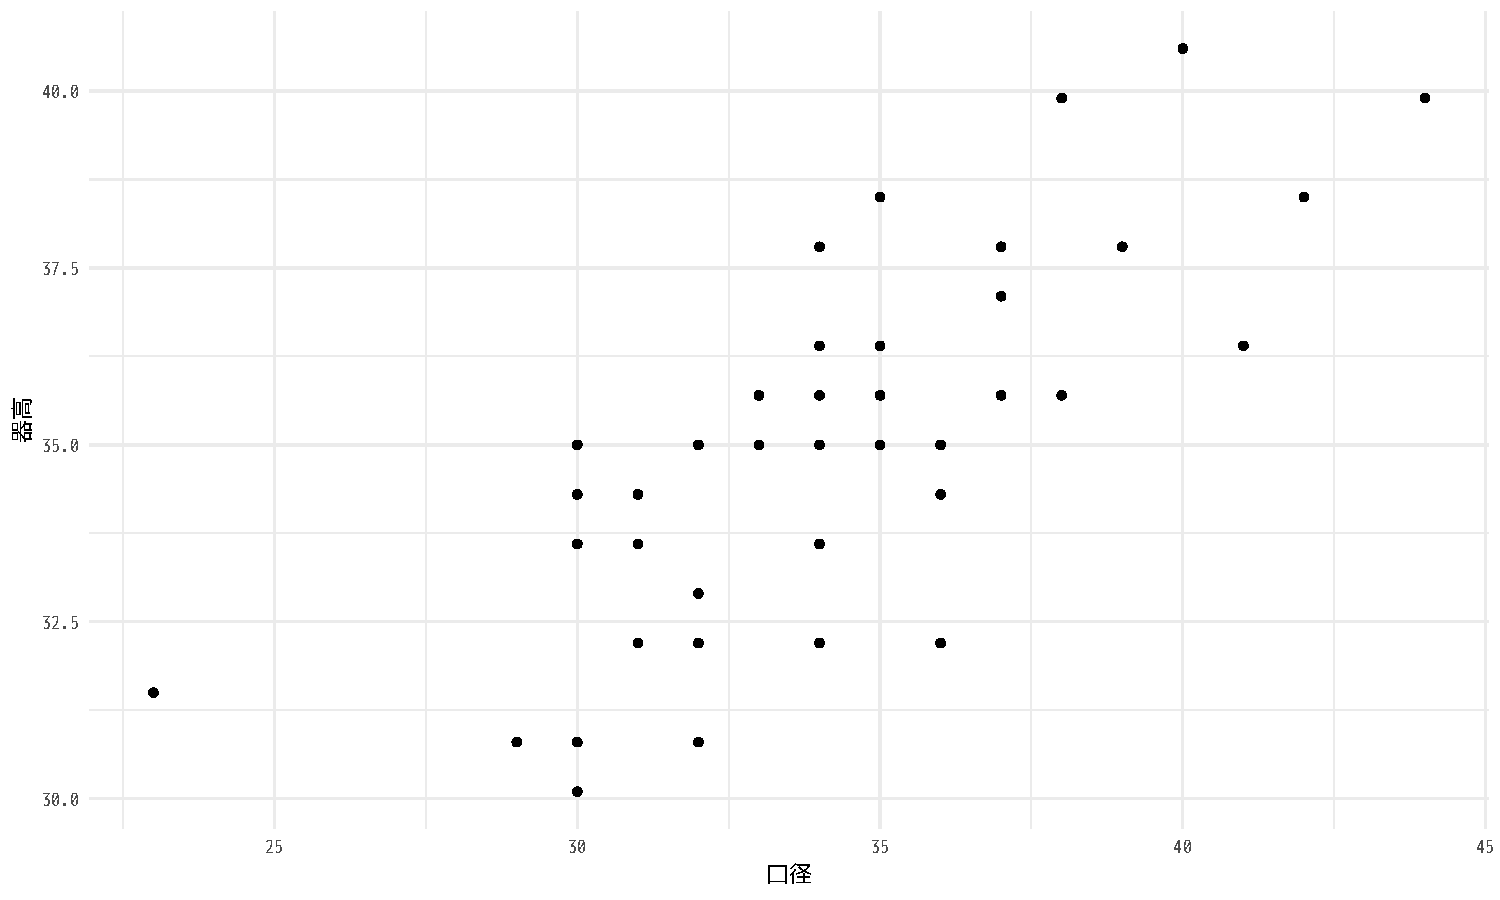
\includegraphics{document_files/figure-latex/unnamed-chunk-23-1.pdf}

どちらかといえば、直線的な分布に見えます。
一次式を当てはめると以下のようになります。

\begin{Shaded}
\begin{Highlighting}[]
\NormalTok{p<-pot}\OperatorTok\KeywordTok{filter}\NormalTok{(分類}\OperatorTok{==}\StringTok{"A型"}\NormalTok{)}\OperatorTok
\StringTok{    }\KeywordTok{ggplot}\NormalTok{(}\KeywordTok{aes}\NormalTok{(}\DataTypeTok{x=}\NormalTok{口径,}\DataTypeTok{y=}\NormalTok{器高))}\OperatorTok{+}
\StringTok{        }\KeywordTok{geom_point}\NormalTok{()}\OperatorTok{+}
\StringTok{        }\KeywordTok{geom_smooth}\NormalTok{(}\DataTypeTok{method=}\StringTok{"lm"}\NormalTok{)}\OperatorTok{+}
\StringTok{        }\KeywordTok{theme_minimal}\NormalTok{()}
\KeywordTok{print}\NormalTok{(p)}
\end{Highlighting}
\end{Shaded}

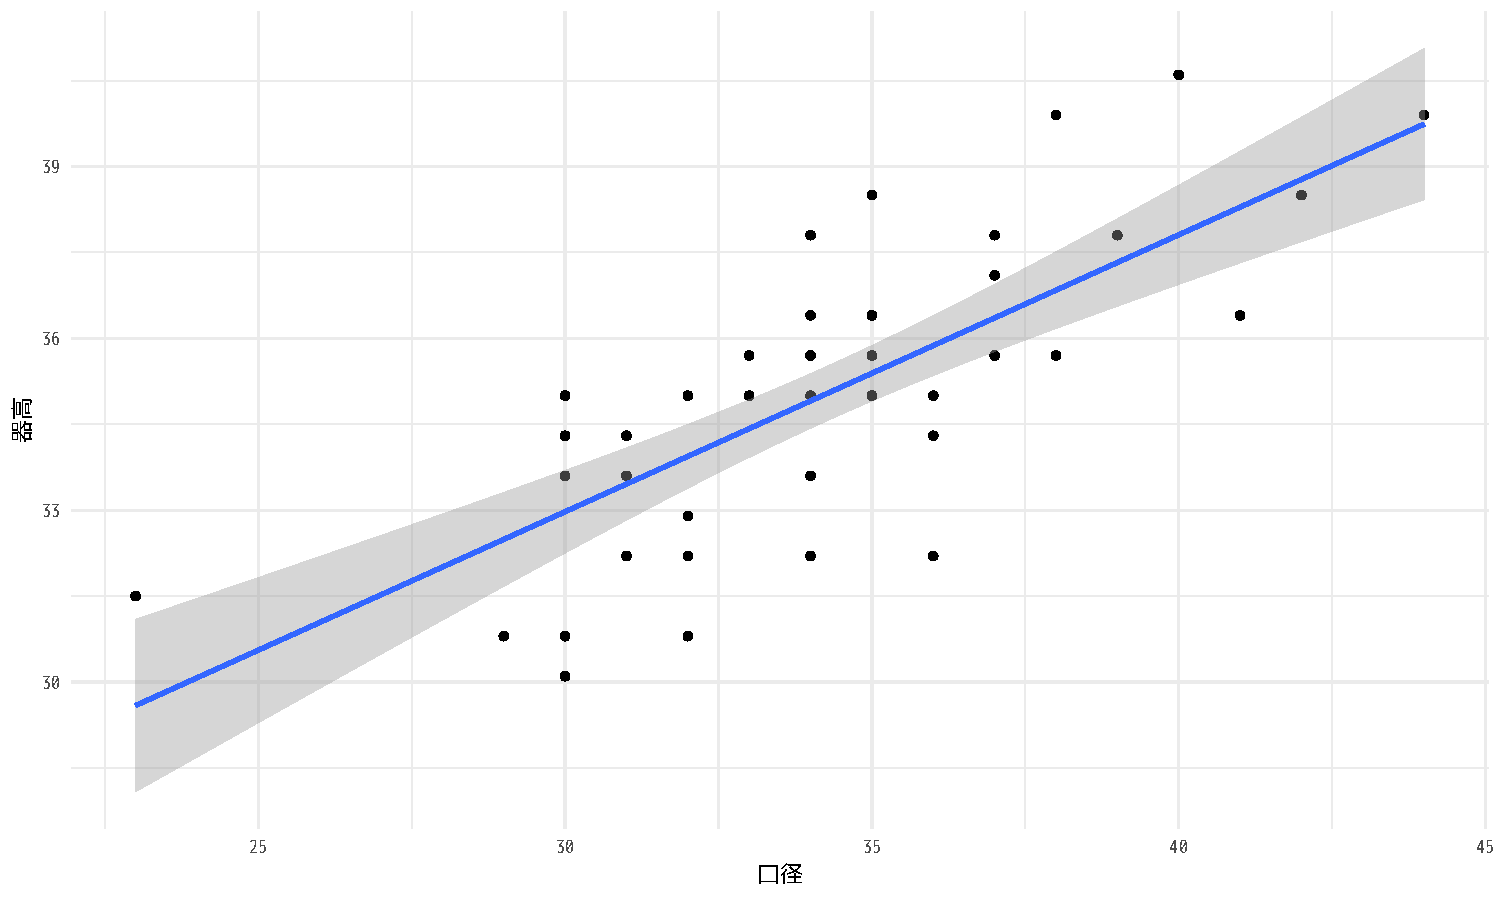
\includegraphics{document_files/figure-latex/unnamed-chunk-24-1.pdf}

上で当てはめた一次式は下のようにして求められます。

\begin{Shaded}
\begin{Highlighting}[]
\NormalTok{coe<-}\KeywordTok{lm}\NormalTok{(器高 }\OperatorTok{~}\StringTok{ }\NormalTok{口径,}\DataTypeTok{data=}\KeywordTok{subset}\NormalTok{(pot,分類}\OperatorTok{==}\StringTok{"A型"}\NormalTok{))}\OperatorTok\KeywordTok{summary}\NormalTok{()}
\NormalTok{coe}\OperatorTok{$}\NormalTok{coefficients}\OperatorTok\KeywordTok{kable}\NormalTok{()}
\end{Highlighting}
\end{Shaded}

\begin{longtable}[]{@{}lrrrr@{}}
\toprule
& Estimate & Std. Error & t value &
Pr(\textgreater{}\textbar{}t\textbar{})\tabularnewline
\midrule
\endhead
(Intercept) & 18.4730087 & 2.1701002 & 8.512514 & 0\tabularnewline
口径 & 0.4833428 & 0.0629292 & 7.680738 & 0\tabularnewline
\bottomrule
\end{longtable}

一次式に当てはめると次の式になります。

y=0.48x+18.47

\subsection{因果関係を可視化する}

「二変量の関係を可視化する」ということの目的は、究極的には「因果関係の可視化」です。

たとえば、学力と子どもの環境の因果関係を統計的に考える場合を考えると、「学力テストの点数」という変量「果」に対して「因」となる変量は「親の収入」や「TVの視聴時間」、「睡眠時間」などが考えられます。

したがって、散布図を描く前に考えることは「因果」の「因」にあたる変量と「果」に当たる変量が何か、ということです。
少なくとも「果」にあたる変量がはっきりしないデータは散布図を描く価値はない、と断言できます。

\subsection{独立変数と従属変数}

散布図を描く場合の約束として、因果関係の「果」にあたるy軸に、「因」にあたる変量をx軸に割り当てます。
y軸に割り当てられた「果」にあたる変量を\textbf{従属変数}、x軸に割り当てられた「因」にあたる変量を\textbf{独立変数}と呼びます。

\subsection{刀身長はどうやって決まるか}

\subsubsection{散布図行列}

恵庭西島松5遺跡出土の古代刀剣を対象としたデータで散布図を作成します。
追求すべきテーマは「刀身長と他の属性との因果関係」です。

刀身の長さは端的に刀剣のサイズを示すものです。
刀剣をつくるときには、まず刀身長が最初に決まり、刀身長に見合った各部のサイズが決められるものと予想されます。

この場合、因果関係の「果」にあたる変量が刀身長であり、「因」にあたる変量を探索することとなります。

GGallyパッケージを利用して散布図行列を描画します。

\begin{Shaded}
\begin{Highlighting}[]
\CommentTok{# GGallyパッケージ読み込み}
\KeywordTok{library}\NormalTok{(GGally)}
\CommentTok{#}
\NormalTok{p<-iron}\OperatorTok\KeywordTok{select}\NormalTok{(全長,刀身長,茎長,刀身先幅,刀身元幅,刀身元厚,茎先幅)}\OperatorTok
\StringTok{    }\KeywordTok{ggpairs}\NormalTok{(}\DataTypeTok{diag=}\KeywordTok{list}\NormalTok{(}\DataTypeTok{continuous=}\StringTok{"barDiag"}\NormalTok{))}
\KeywordTok{print}\NormalTok{(p)}
\end{Highlighting}
\end{Shaded}

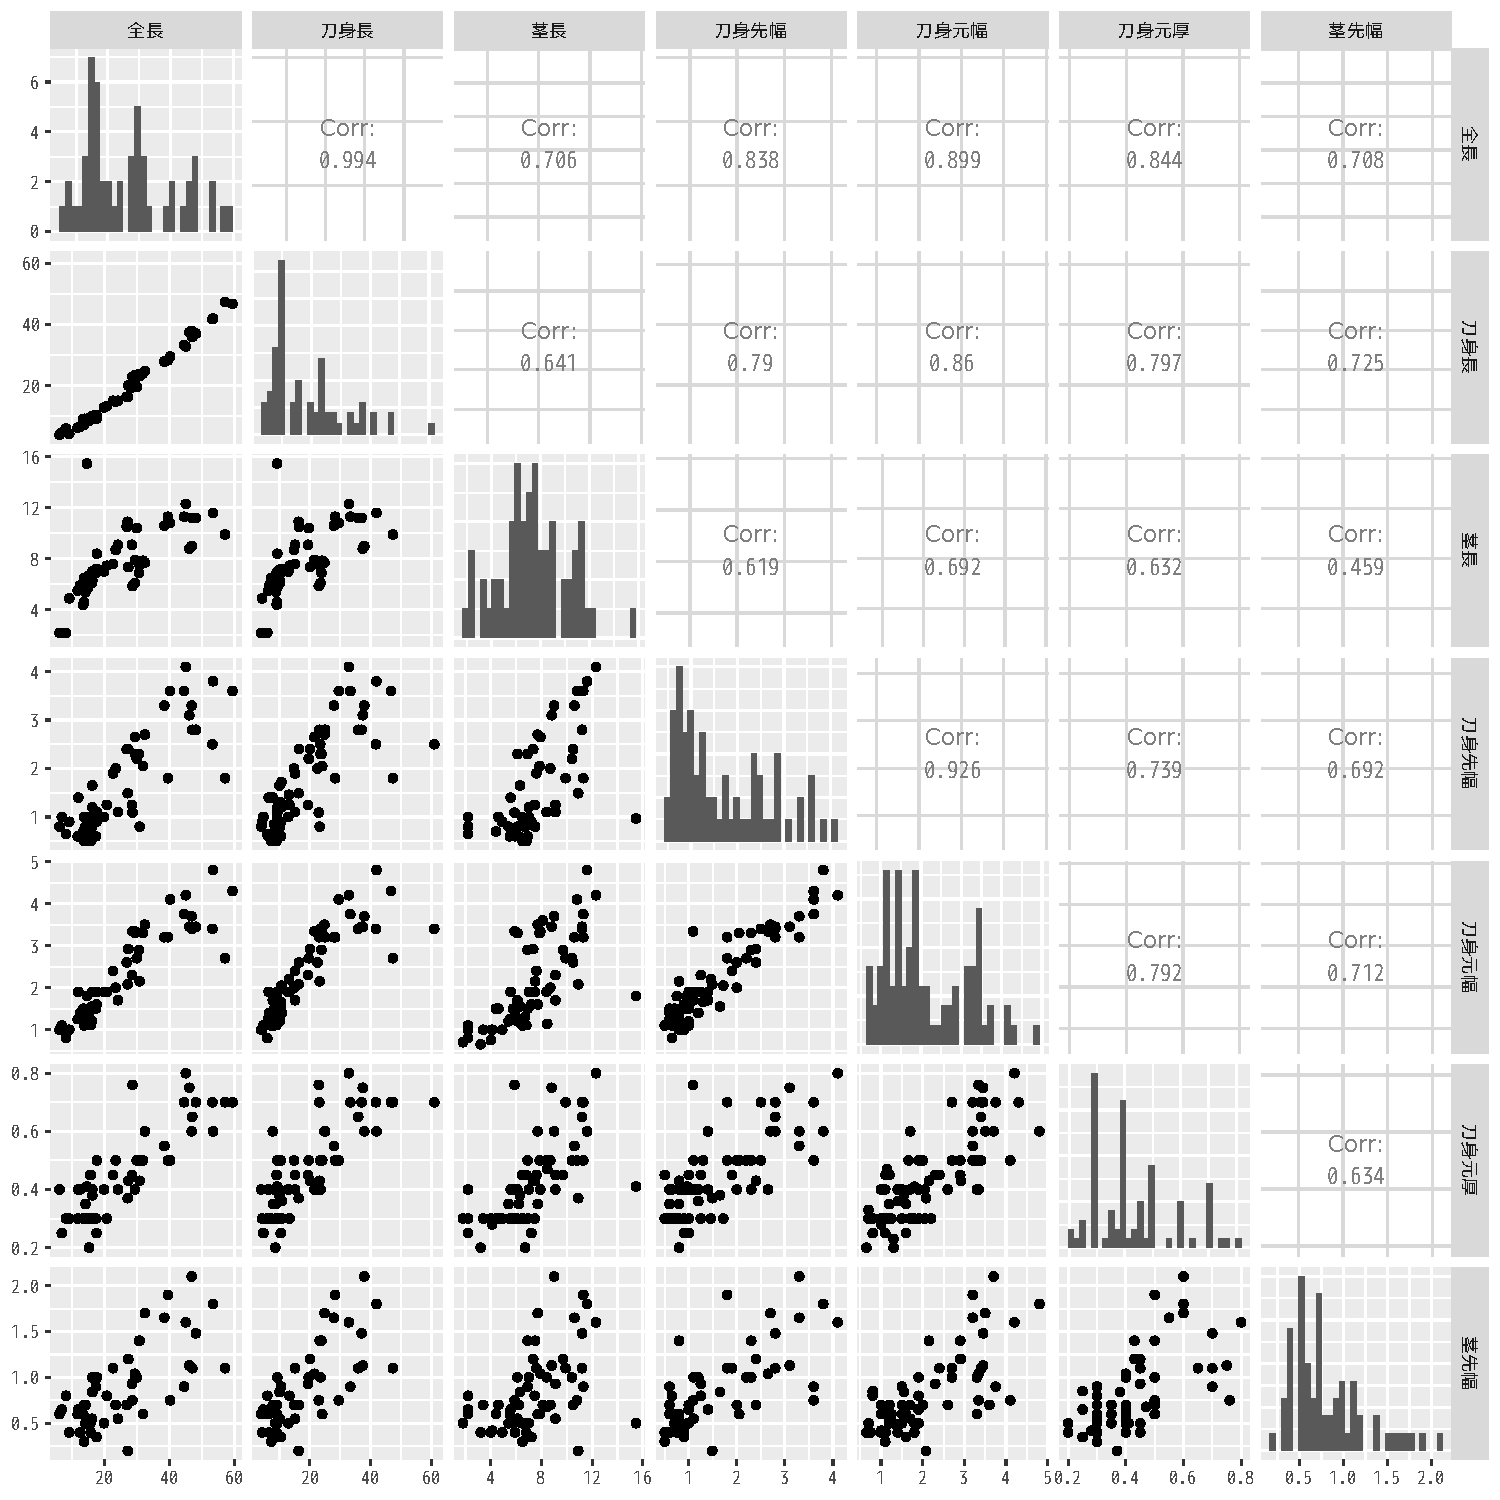
\includegraphics{document_files/figure-latex/unnamed-chunk-26-1.pdf}

散布図が示すところからは、多くの属性が刀身長と相関関係にあることが読み取れます。
一方、刀身元幅のように非常に強い相関を示す変量もあれば、茎先幅のように相関が弱そうな変量もあります。
刀身長との相関の強弱を判断することで、古代剣製作にかかる規範意識を読み取ることが可能かもしれません。

\subsubsection{予測する}

散布図を作成する目的は2変量の因果関係を考えることでした。因果関係がわかるということは\textbf{予測}ができるということです。次は古代刀剣の刀身元幅から刀身長を予測することを検討します。出土刀剣では刀身が破損せずに出土することはまれですから、元幅から刀身長を予測できれば、出土刀剣の把握に大きな成果がありそうです。

\begin{Shaded}
\begin{Highlighting}[]
\NormalTok{p<-iron}\OperatorTok
\StringTok{    }\KeywordTok{ggplot}\NormalTok{(}\KeywordTok{aes}\NormalTok{(}\DataTypeTok{x=}\NormalTok{刀身元幅,}\DataTypeTok{y=}\NormalTok{刀身長))}\OperatorTok{+}
\StringTok{        }\KeywordTok{geom_point}\NormalTok{()}\OperatorTok{+}
\StringTok{        }\KeywordTok{geom_smooth}\NormalTok{(}\DataTypeTok{method=}\StringTok{"lm"}\NormalTok{)}\OperatorTok{+}
\StringTok{        }\KeywordTok{theme_minimal}\NormalTok{()}
\KeywordTok{print}\NormalTok{(p)}
\end{Highlighting}
\end{Shaded}

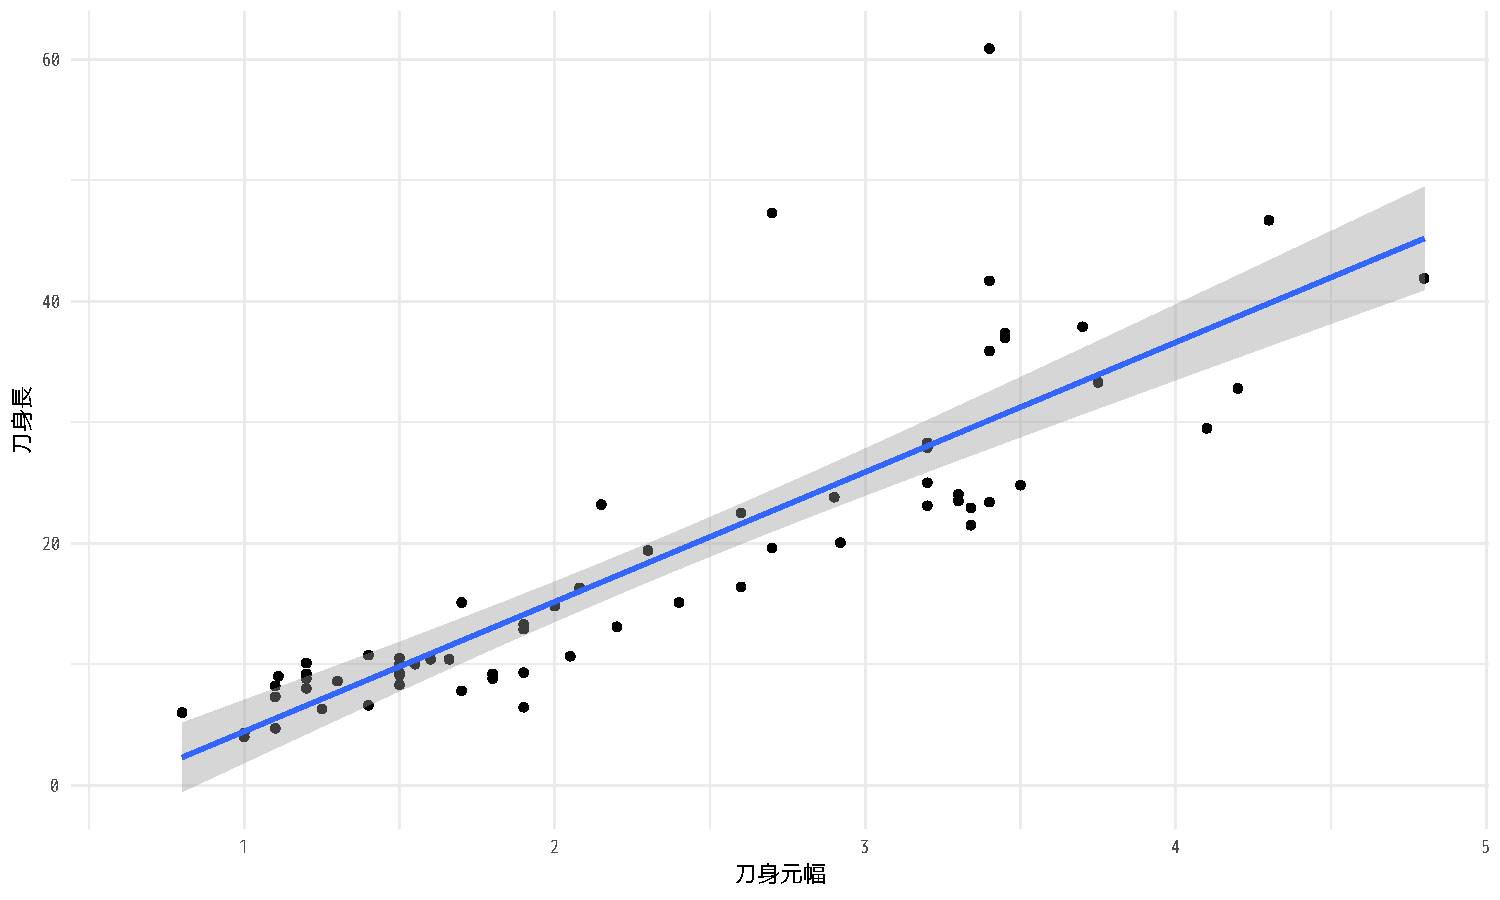
\includegraphics{document_files/figure-latex/unnamed-chunk-27-1.pdf}

なお、刀身元幅を独立変数とする刀身長の予測式は次のとおりです。

\begin{Shaded}
\begin{Highlighting}[]
\NormalTok{icoe<-}\KeywordTok{lm}\NormalTok{(刀身長 }\OperatorTok{~}\StringTok{ }\NormalTok{刀身元幅,}\DataTypeTok{data=}\NormalTok{iron)}\OperatorTok\KeywordTok{summary}\NormalTok{()}
\NormalTok{icoe}\OperatorTok{$}\NormalTok{coefficients}\OperatorTok\KeywordTok{kable}\NormalTok{()}
\end{Highlighting}
\end{Shaded}

\begin{longtable}[]{@{}lrrrr@{}}
\toprule
& Estimate & Std. Error & t value &
Pr(\textgreater{}\textbar{}t\textbar{})\tabularnewline
\midrule
\endhead
(Intercept) & -6.280888 & 1.9780720 & -3.175257 &
0.0022892\tabularnewline
刀身元幅 & 10.723991 & 0.7889999 & 13.591878 & 0.0000000\tabularnewline
\bottomrule
\end{longtable}

y=10.72x-6.28

\hypertarget{-2}{%
\subsection{まとめ}\label{-2}}

\begin{itemize}
\tightlist
\item
  連続量のデータは、まず\textbf{分布}を調べる(ヒストグラムを作成する)
\item
  構成比(離散量)のデータに円グラフは使わない(棒グラフを使う)
\item
  連続量どうしの関係は散布図で可視化する
\end{itemize}

この 記事 は クリエイティブ・コモンズ 表示 4.0 国際
ライセンスの下に提供されています。


\end{document}
